\chapter{Transformer的理论基础}


\label{cha:sysu-thesis-latex-install-guide}
\section{transformer的简介}

Transformer是最早在自然语言处理领域提出并逐渐被广泛运用于其他领域的神经网络模型。Transformer的出现在性能上超越了很多传统的自然语言处理模型如RNN、LSTM等。并且Transformer还具有突破了并行计算的限制、更具可解释性等优点。

在最开始的使用中,transformer包括encoding(编码器)和decoding(解码器)两个部分。其神经网络的结构如图\ref{img301}所示:

\begin{figure}[h]
	\centering
	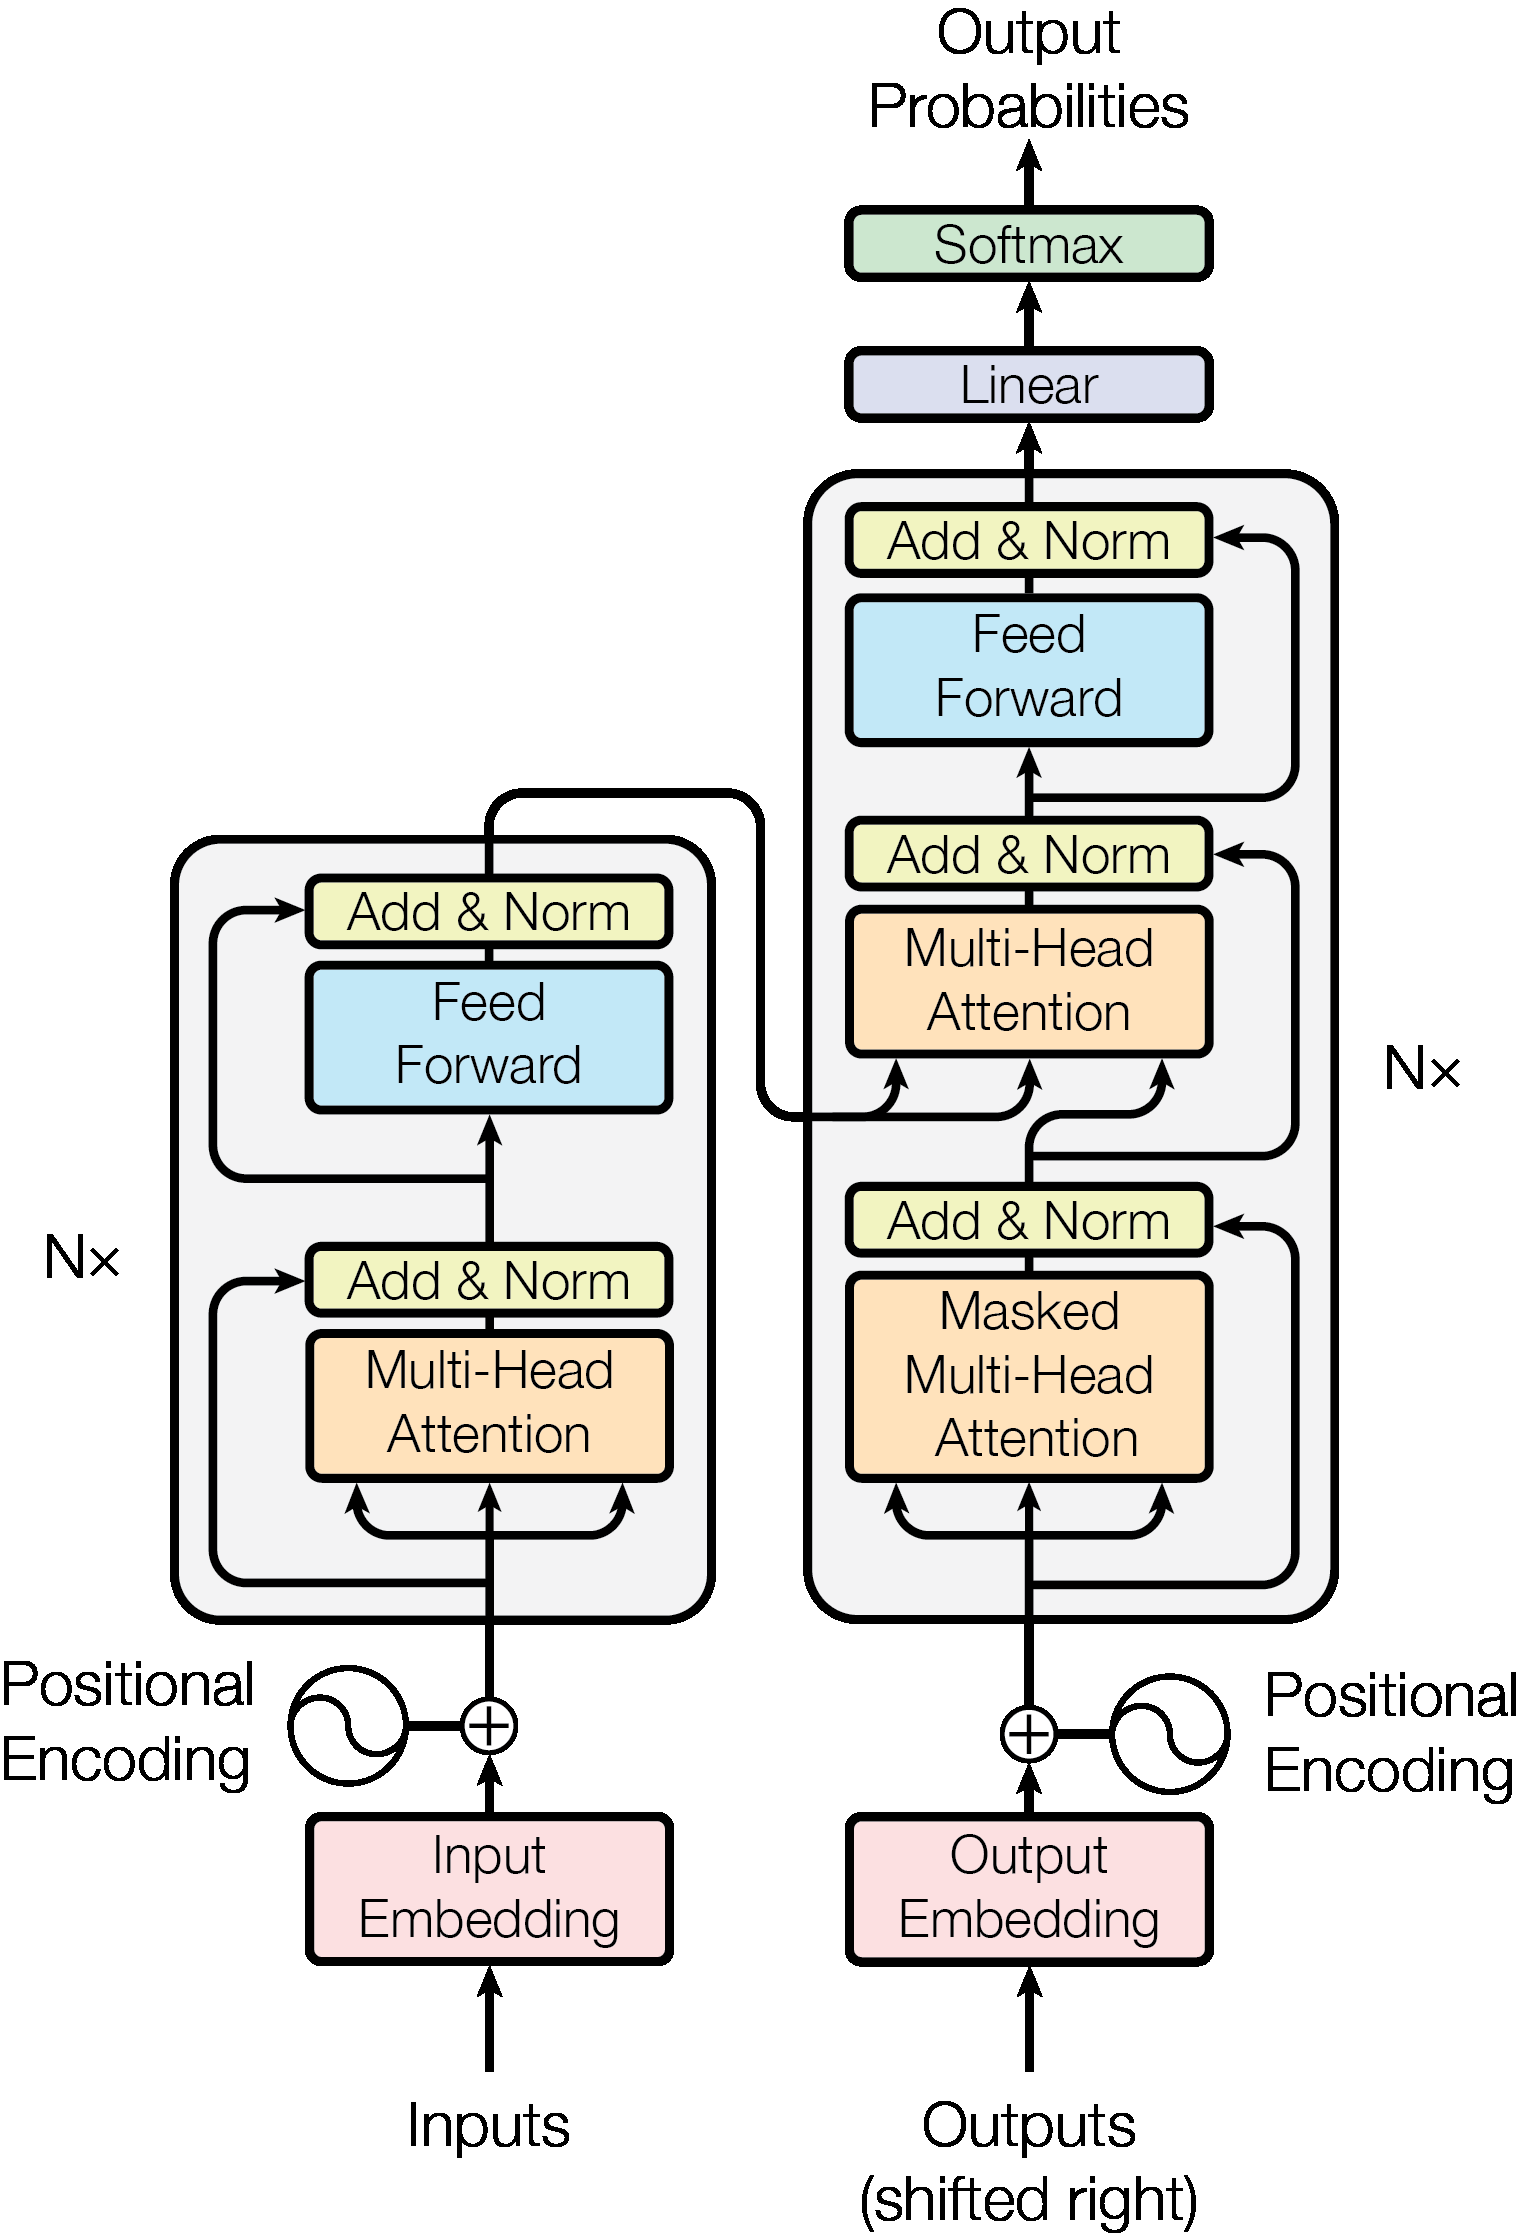
\includegraphics[width=0.4\columnwidth]{image/chap03/img301.png}
	\caption{"Attention Is All You Need"中的Transformer模型\cite{vaswani2017attention}}
	\label{img301}
\end{figure}

\section{自注意力机制}
\subsection{注意力机制的原理}
注意力机制是Transformer的核心机制。自注意力机制的提出是对人类获取外界信息的机制的一种抽象。当我们观察外界信息,并不是对外界的所有信息“全盘吸收”,而是会无意识地忽略某些“不重要”的信息,从而能提高对外界信息的吸收效率。我们用一个机器翻译的任务来阐述注意力机制的原理。

\begin{figure}[h]
	\begin{minipage}[t]{0.5\linewidth}
		\centering
		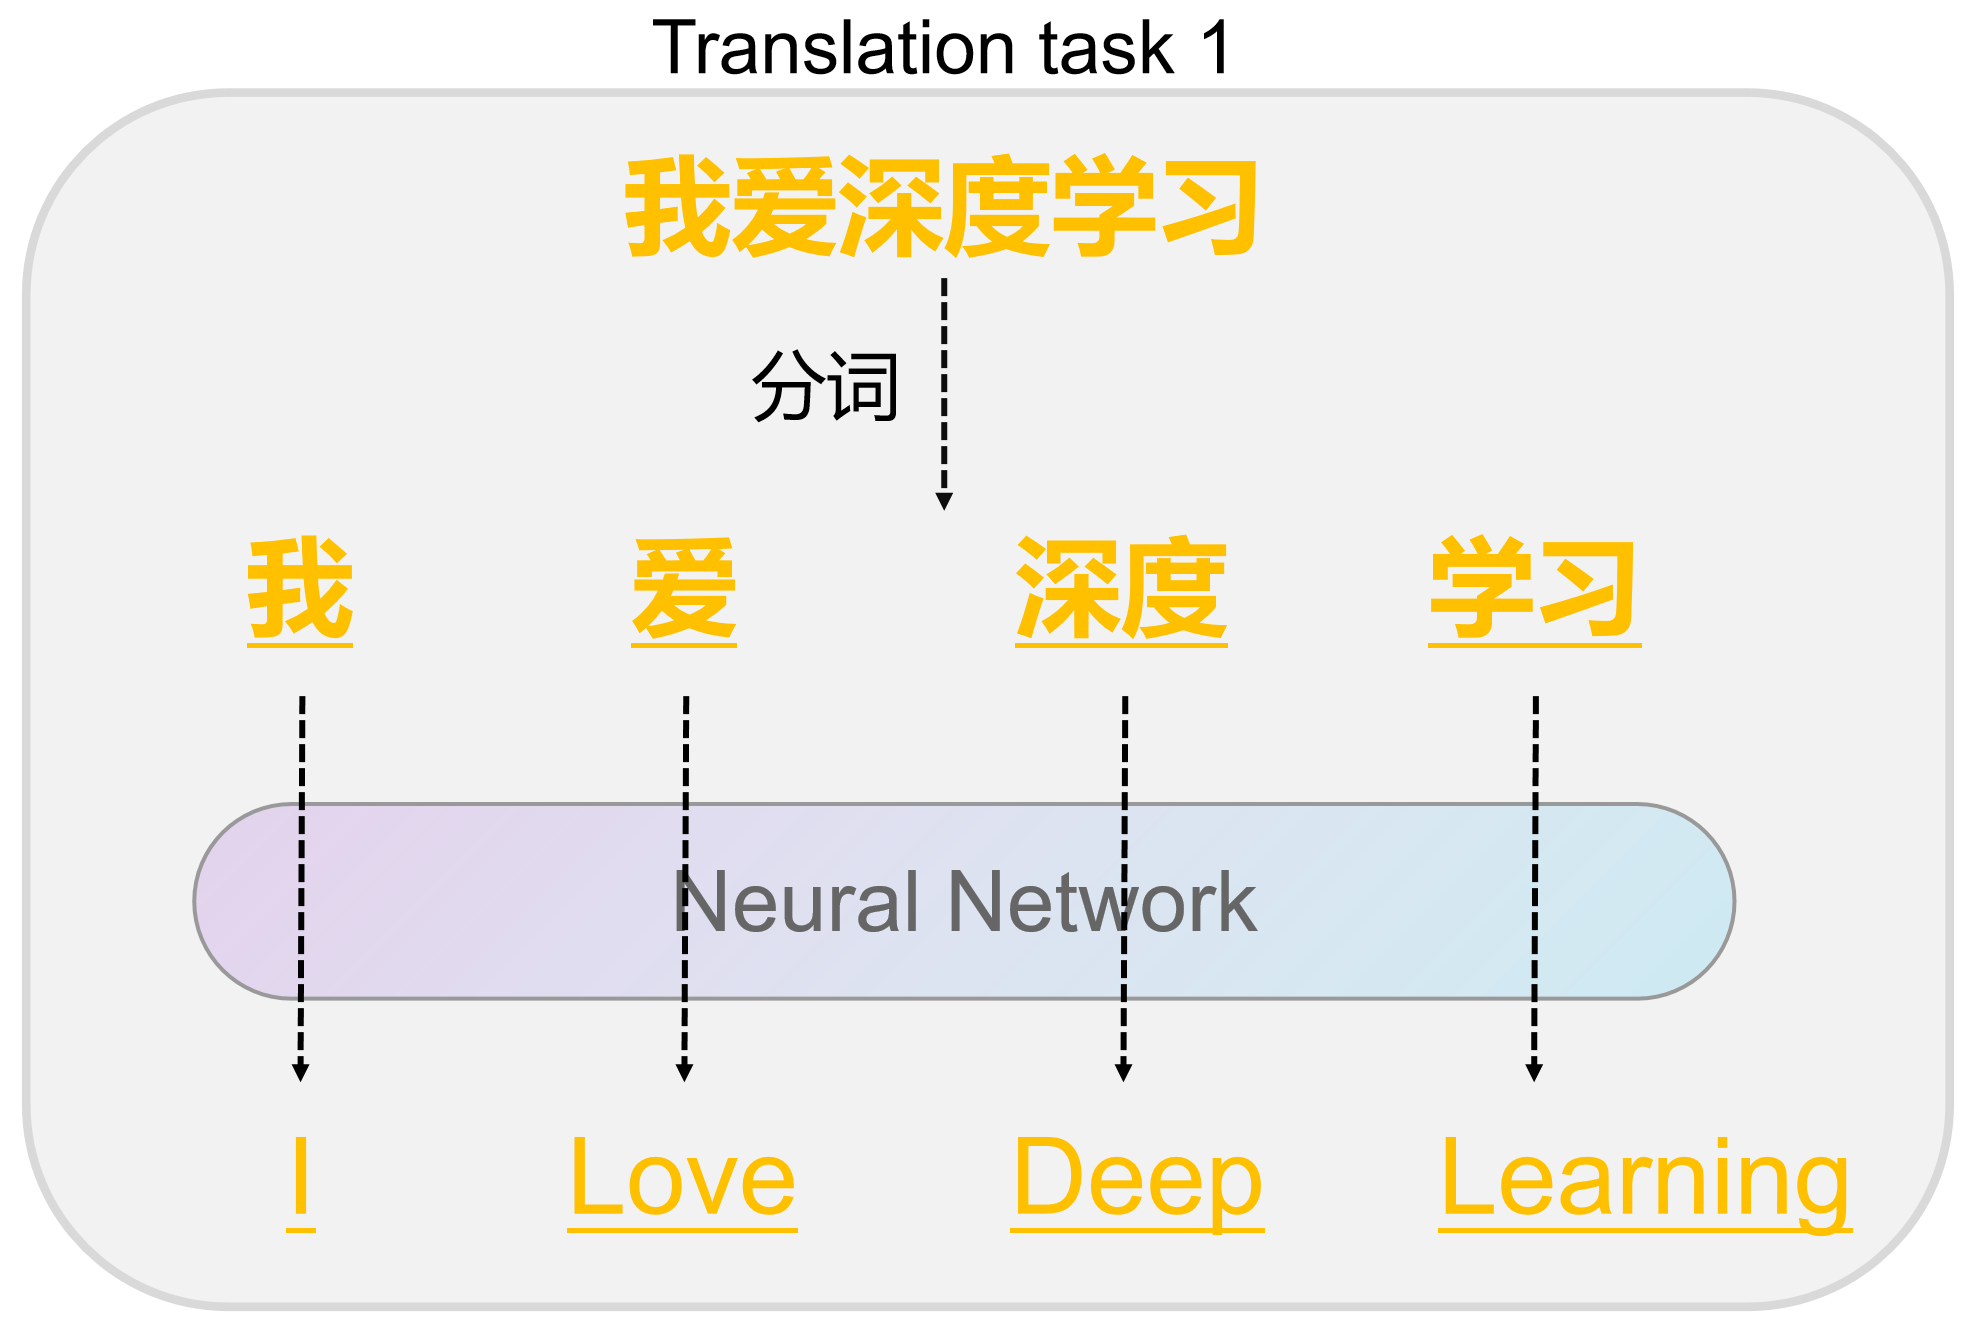
\includegraphics[scale=0.25]{image/chap03/img302.png}
		\caption{翻译任务1}
		\label{img302}
	\end{minipage}%
	\begin{minipage}[t]{0.5\linewidth}
		\centering
		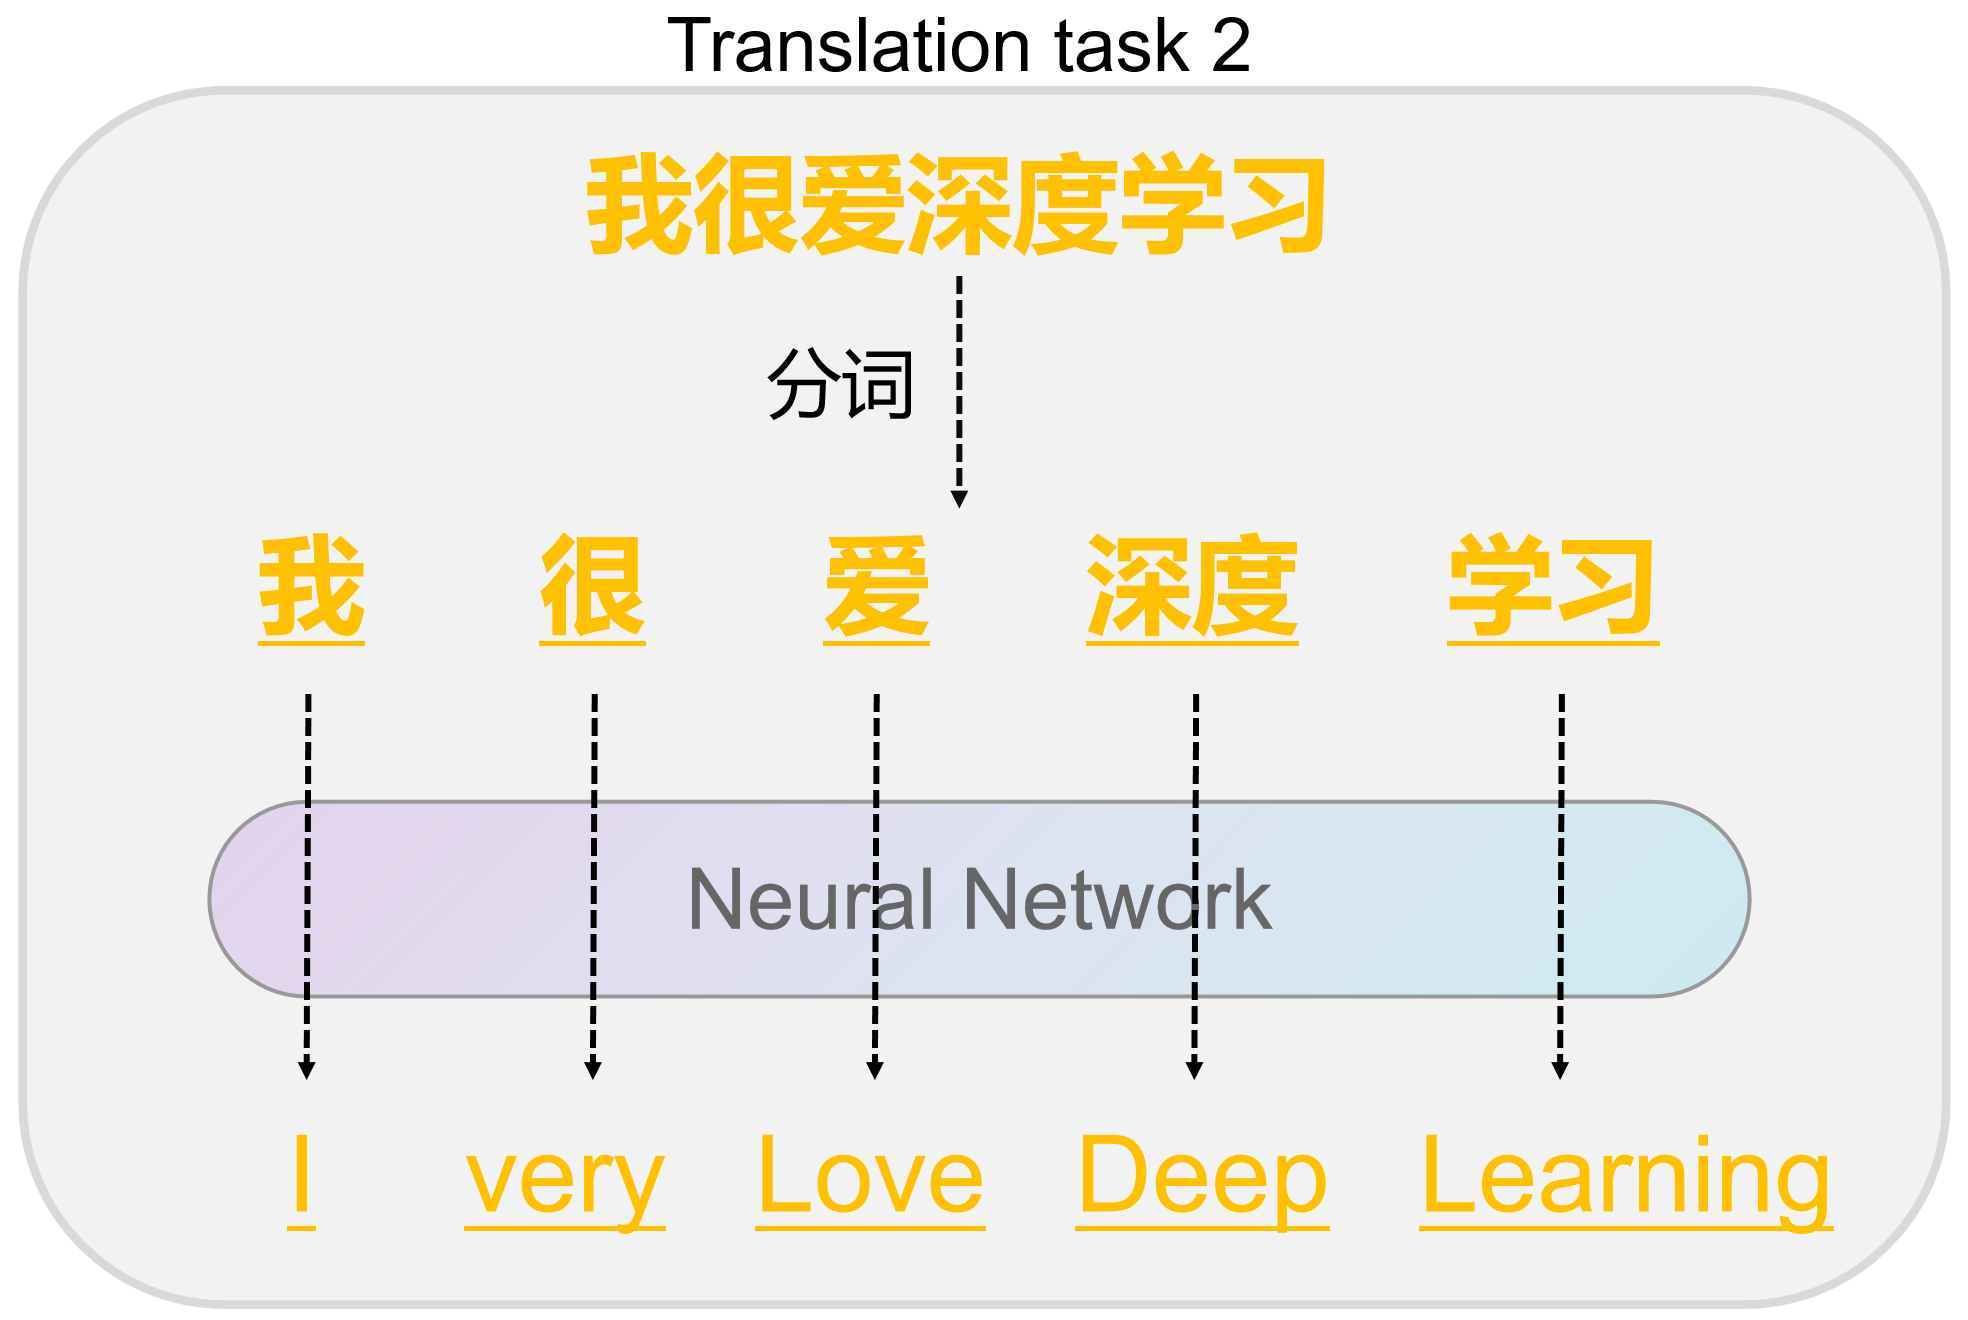
\includegraphics[scale=0.25]{image/chap03/img303.png}
		\caption{翻译任务2}
		\label{img303}
	\end{minipage}
\end{figure}

假设我们要使用神经网络来完成中译英的机器翻译任务。如果完全不考虑整个句子的上下文信息,那么机器翻译其实就是训练神经网络,使其能将特定的中文字符映射到特定的英文字符,这时只需采用最简单的Mlp神经网络就能实现这种功能。这种做法在某些机器翻译任务中是可行的,如图\ref{img302}。但在大多数的机器翻译任务中,这种直接映射的做法会导致语法上的错误或语义上的歧义,如图\ref{img303}的机器翻译任务。

这时,在翻译单个词时,通过结合上下文信息再进行翻译就十分重要了。而Transformer中的注意力机制就能很好地实现上下文信息的结合。首先在进行机器翻译的任务之前,都会对翻译的单词进行“编码”使其能被计算机运算与处理。比如将四字句子“我”“很”“爱”“深度”“学习”编码成五个向量$x_1,x_2,x_3,x_4,x_5$。并记$X=[x_1,x_2,x_3,x_4,x_5]$代表整个句子,即如图\ref{img304}所示.

\begin{figure}[h]
	\centering
	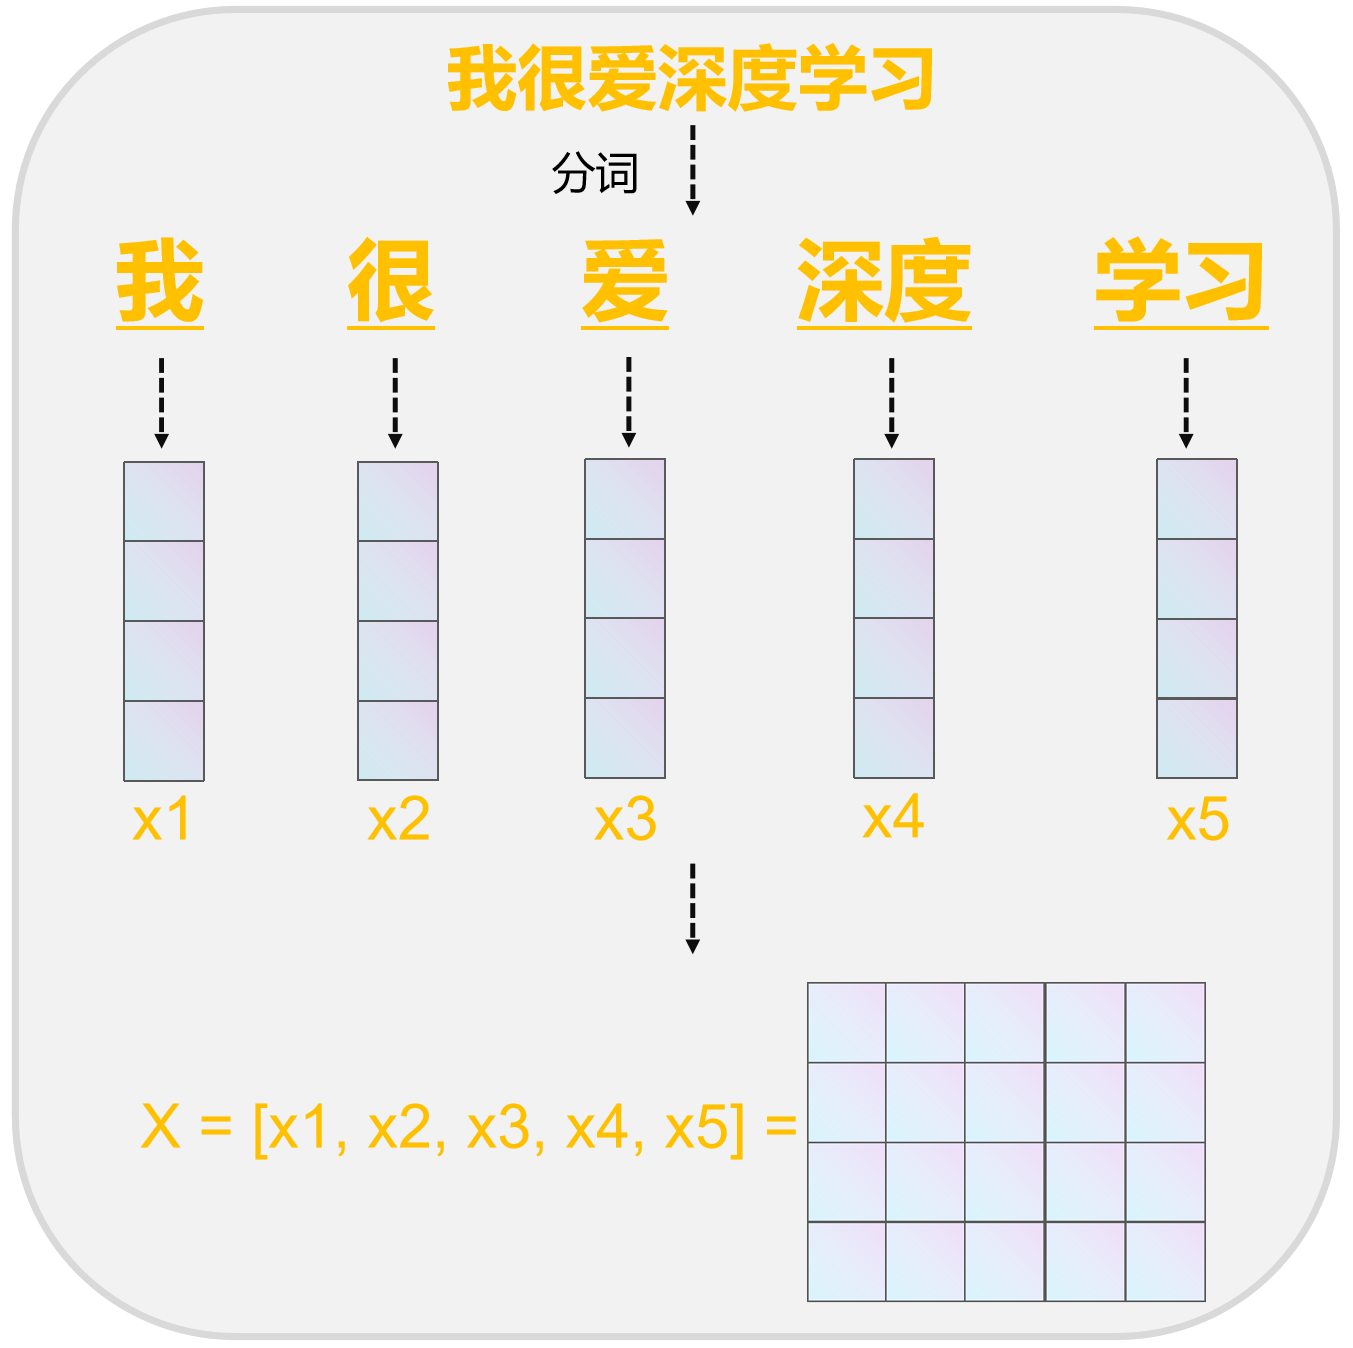
\includegraphics[width=0.4\columnwidth]{image/chap03/img304.png}
	\caption{自然语言编码过程}
	\label{img304}
\end{figure}

 在翻译词“很”的时候,我们想知道所在句子中的其他词所提供的信息量的程度。我们需要找到一个值域为$[ 0, 1]$的注意力打分函数$F$,来衡量这种提供信息的权重。即若我们输入$F($“很”,“我”$)=$$F(x_2,x_1)=\omega_{21}$,所得到的$\omega_{21}$代表在翻译“很”字时,“我”字所提供信息的权重。以此类推,我们可以得到各个字在翻译“很”字时提供的信息权重$\omega_{21},\omega_{22},\omega_{23},\omega_{24},\omega_{25}$,即:

\begin{equation} \label{301}
\left\{
\begin{array}{l}
	F(\vec{x_2},\vec{x_1})=\omega_{21}\\
	F(\vec{x_2},\vec{x_2})=\omega_{22}\\
	\qquad \qquad \ \ \vdots\\
	F(\vec{x_2},\vec{x_5})=\omega_{25}
\end{array}
\right.
\end{equation}

\begin{figure}[h]
	\begin{minipage}[t]{0.5\linewidth}
		\centering
		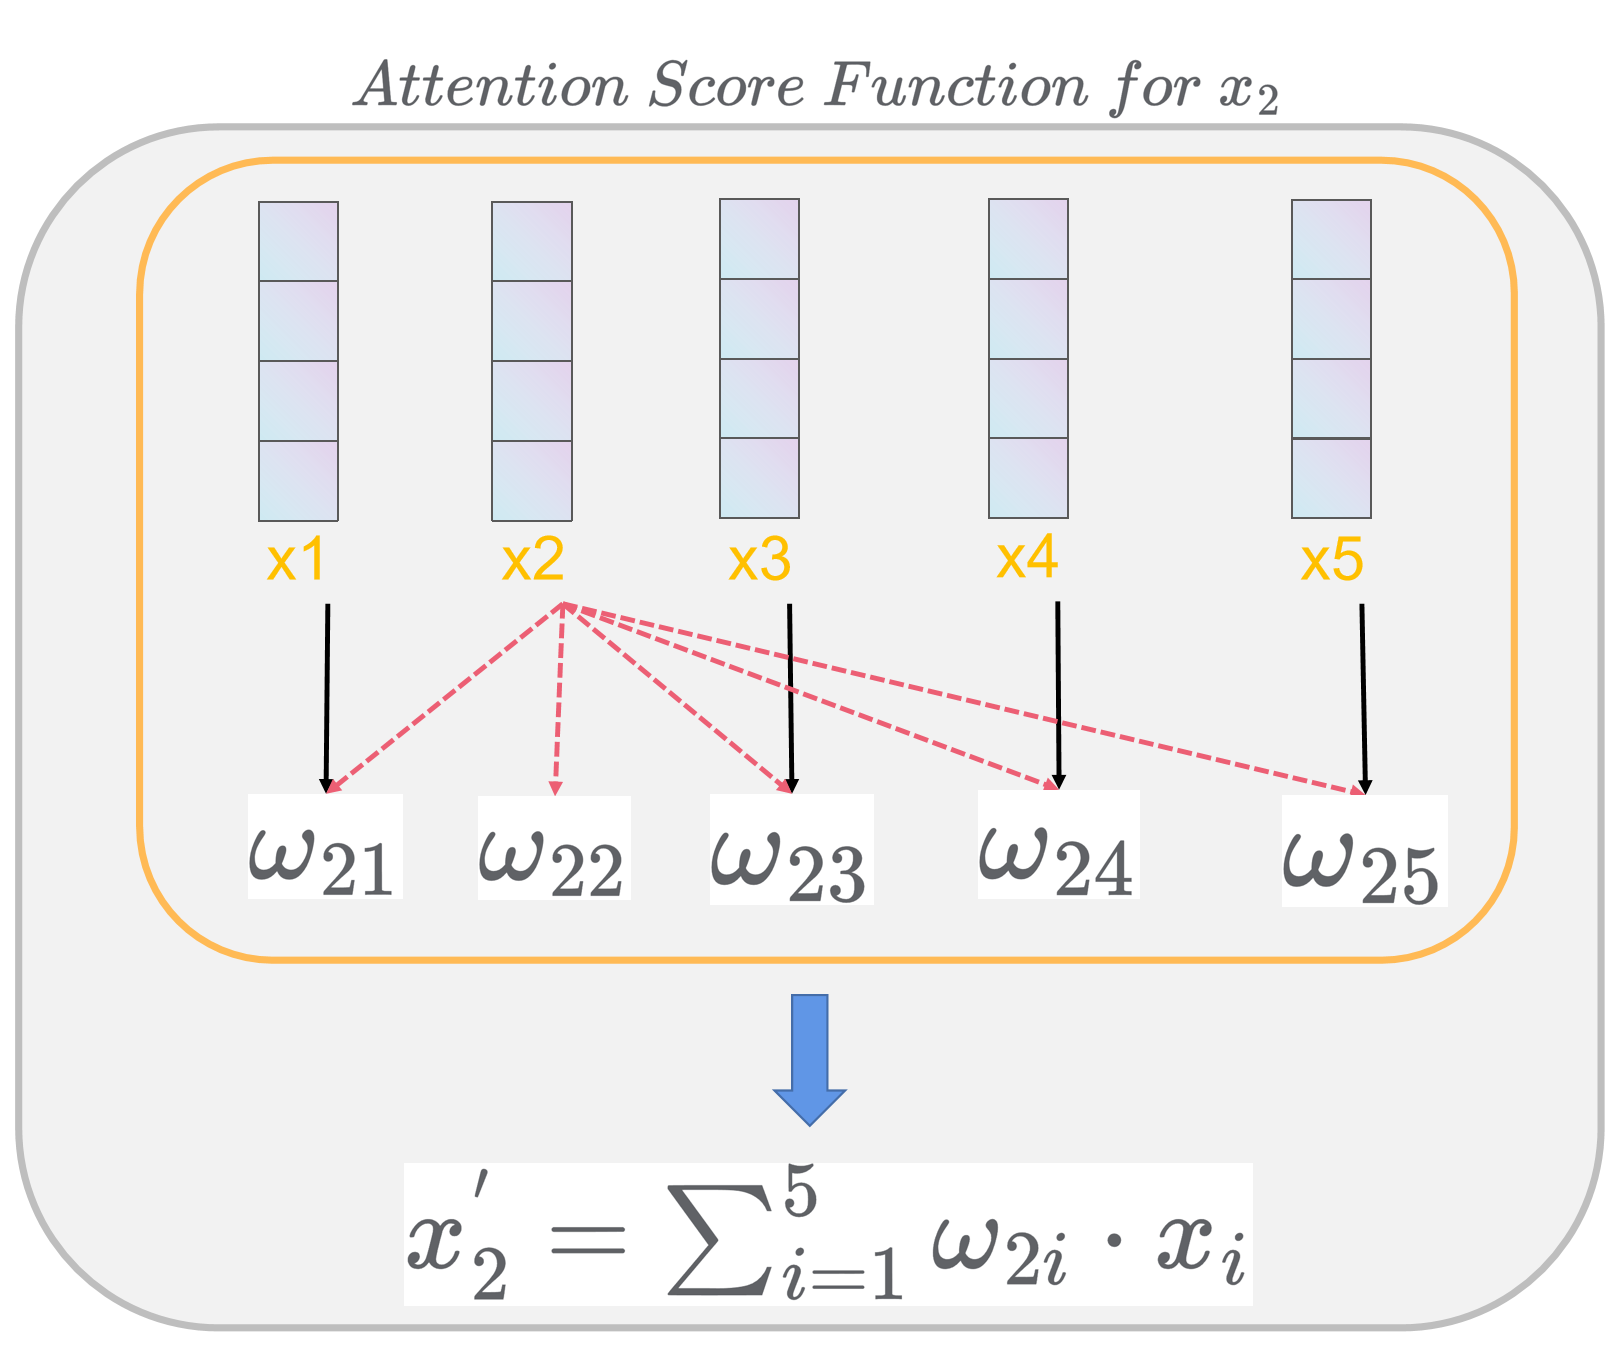
\includegraphics[scale=0.25]{image/chap03/img305.png}
		\caption{注意力机制的原理}
		\label{img305}
	\end{minipage}%
	\begin{minipage}[t]{0.5\linewidth}
		\centering
		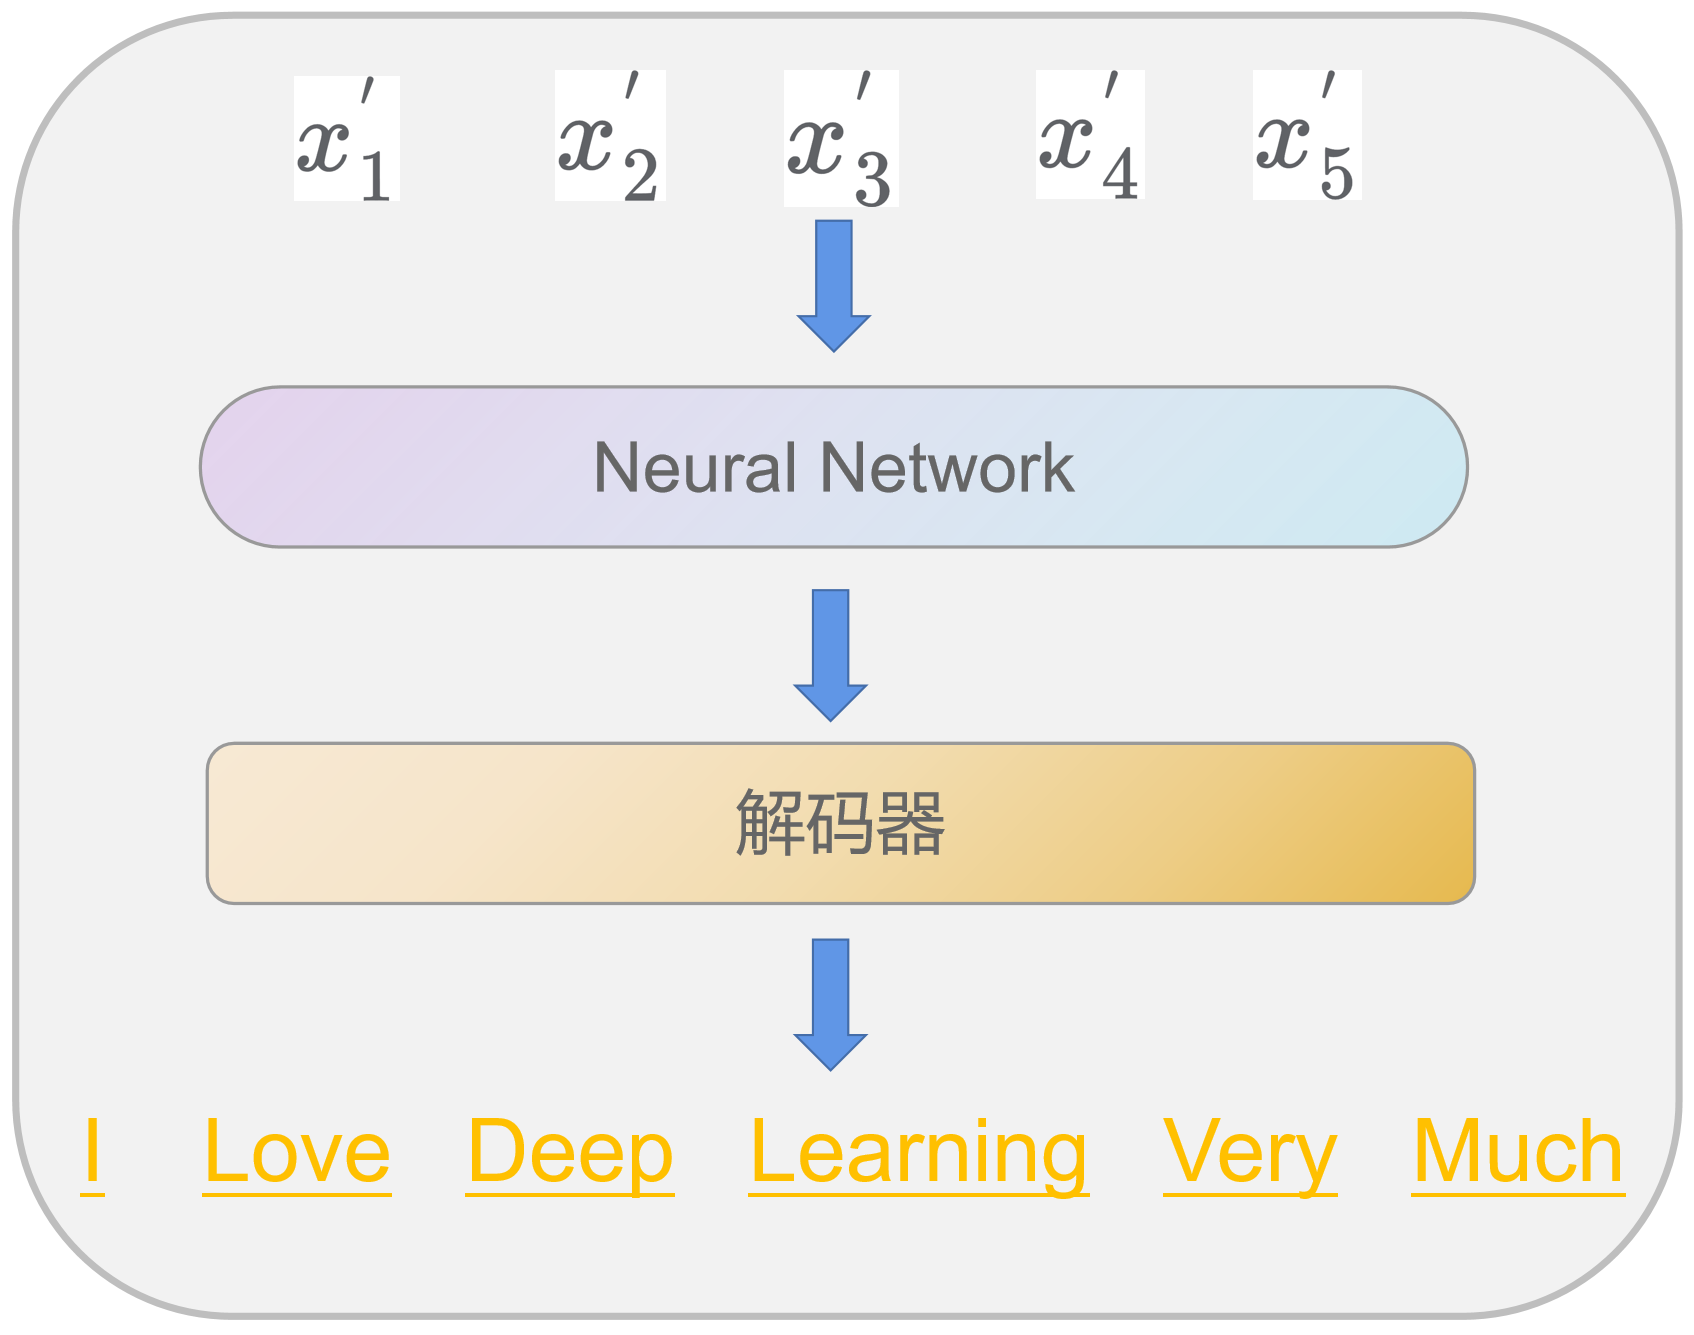
\includegraphics[scale=0.25]{image/chap03/img306.png}
		\caption{自然语言解码过程}
		\label{img306}
	\end{minipage}
\end{figure}

这时根据注意力权重进行加权求和得到的$x_2^{'} = \omega_{21}x_{1}+\omega_{22}x_{2}+\omega_{23}x_{3}+\omega_{24}x_{4}+\omega_{25}x_{5}$就能代表结合了上下文信息后的“很”字,如图\ref{img305}。同样的步骤,我们能得到结合了全局信息的$x_1^{'},…,x_5^{'}$,将其作为神经网络的输入,就能得到考虑了上下文信息的翻译,如图\ref{img306}。

机器翻译的Transformer模型就是上述的三个步骤的相互组合,如图\ref{img307}。

\begin{figure}[h]
	\centering
	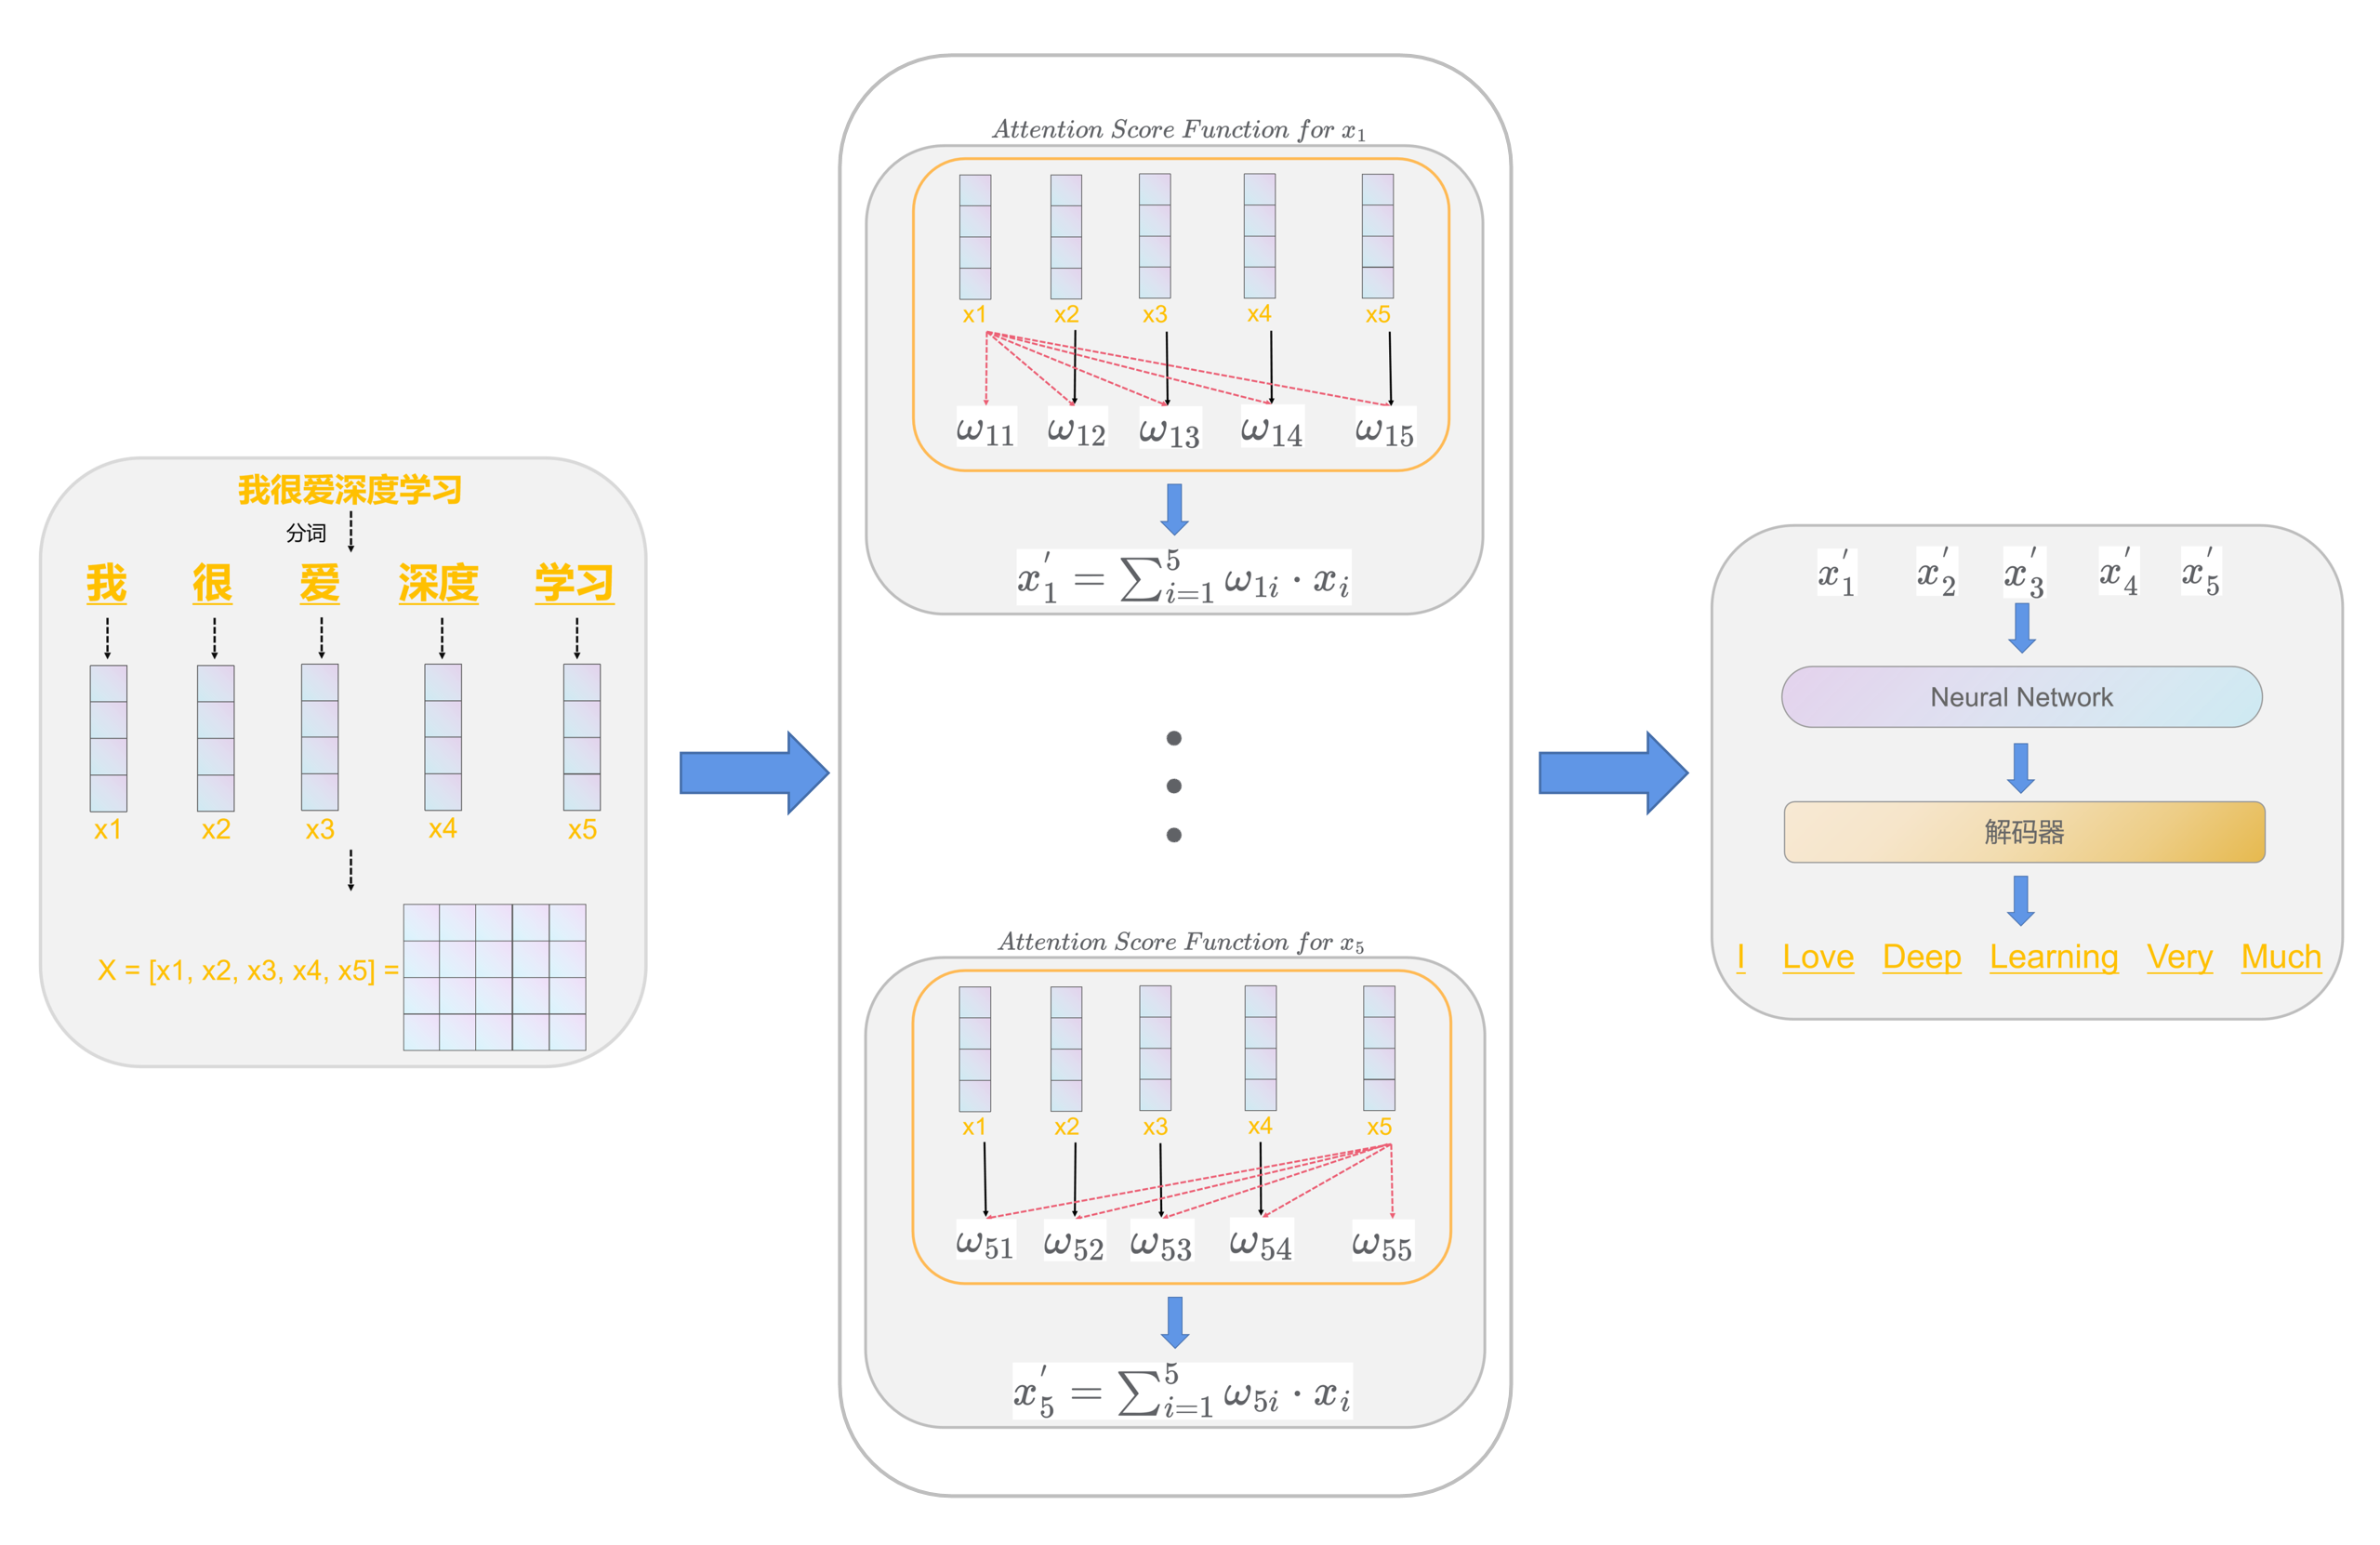
\includegraphics[width=0.9\columnwidth]{image/chap03/img307.png}
	\caption{运用注意力机制的机器翻译过程}
	\label{img307}
\end{figure}



\subsection{自注意力机制的实现}

自注意力机制的运算实现主要分成四个部分:

\subsubsection{将$X$经过三个线性变换后得到$Q,K,V$}

将多个研究对象进行编码后得到的的向量$x_1,\cdots ,x_n$(在如图\ref{img303}所示的任务中,$x_1,\cdots ,x_5$分别代表“我”“很”“爱”“深度”“学习”五个单词),将其按行排列而成的矩阵记为$X$,如图\ref{img308}左边。$X$矩阵与定义三个线性变换矩阵$W_q,W_k,W_v$相乘得到三个矩阵$Q,K,V$。得到的$Q,K,V$的各行元素各代表$X$矩阵中的一个向量。

其中$W_q,W_k,W_v$为可学习的参数,这一步的目的是为了使注意力打分函数成为可学习的函数。

\begin{figure}[h]
	\centering
	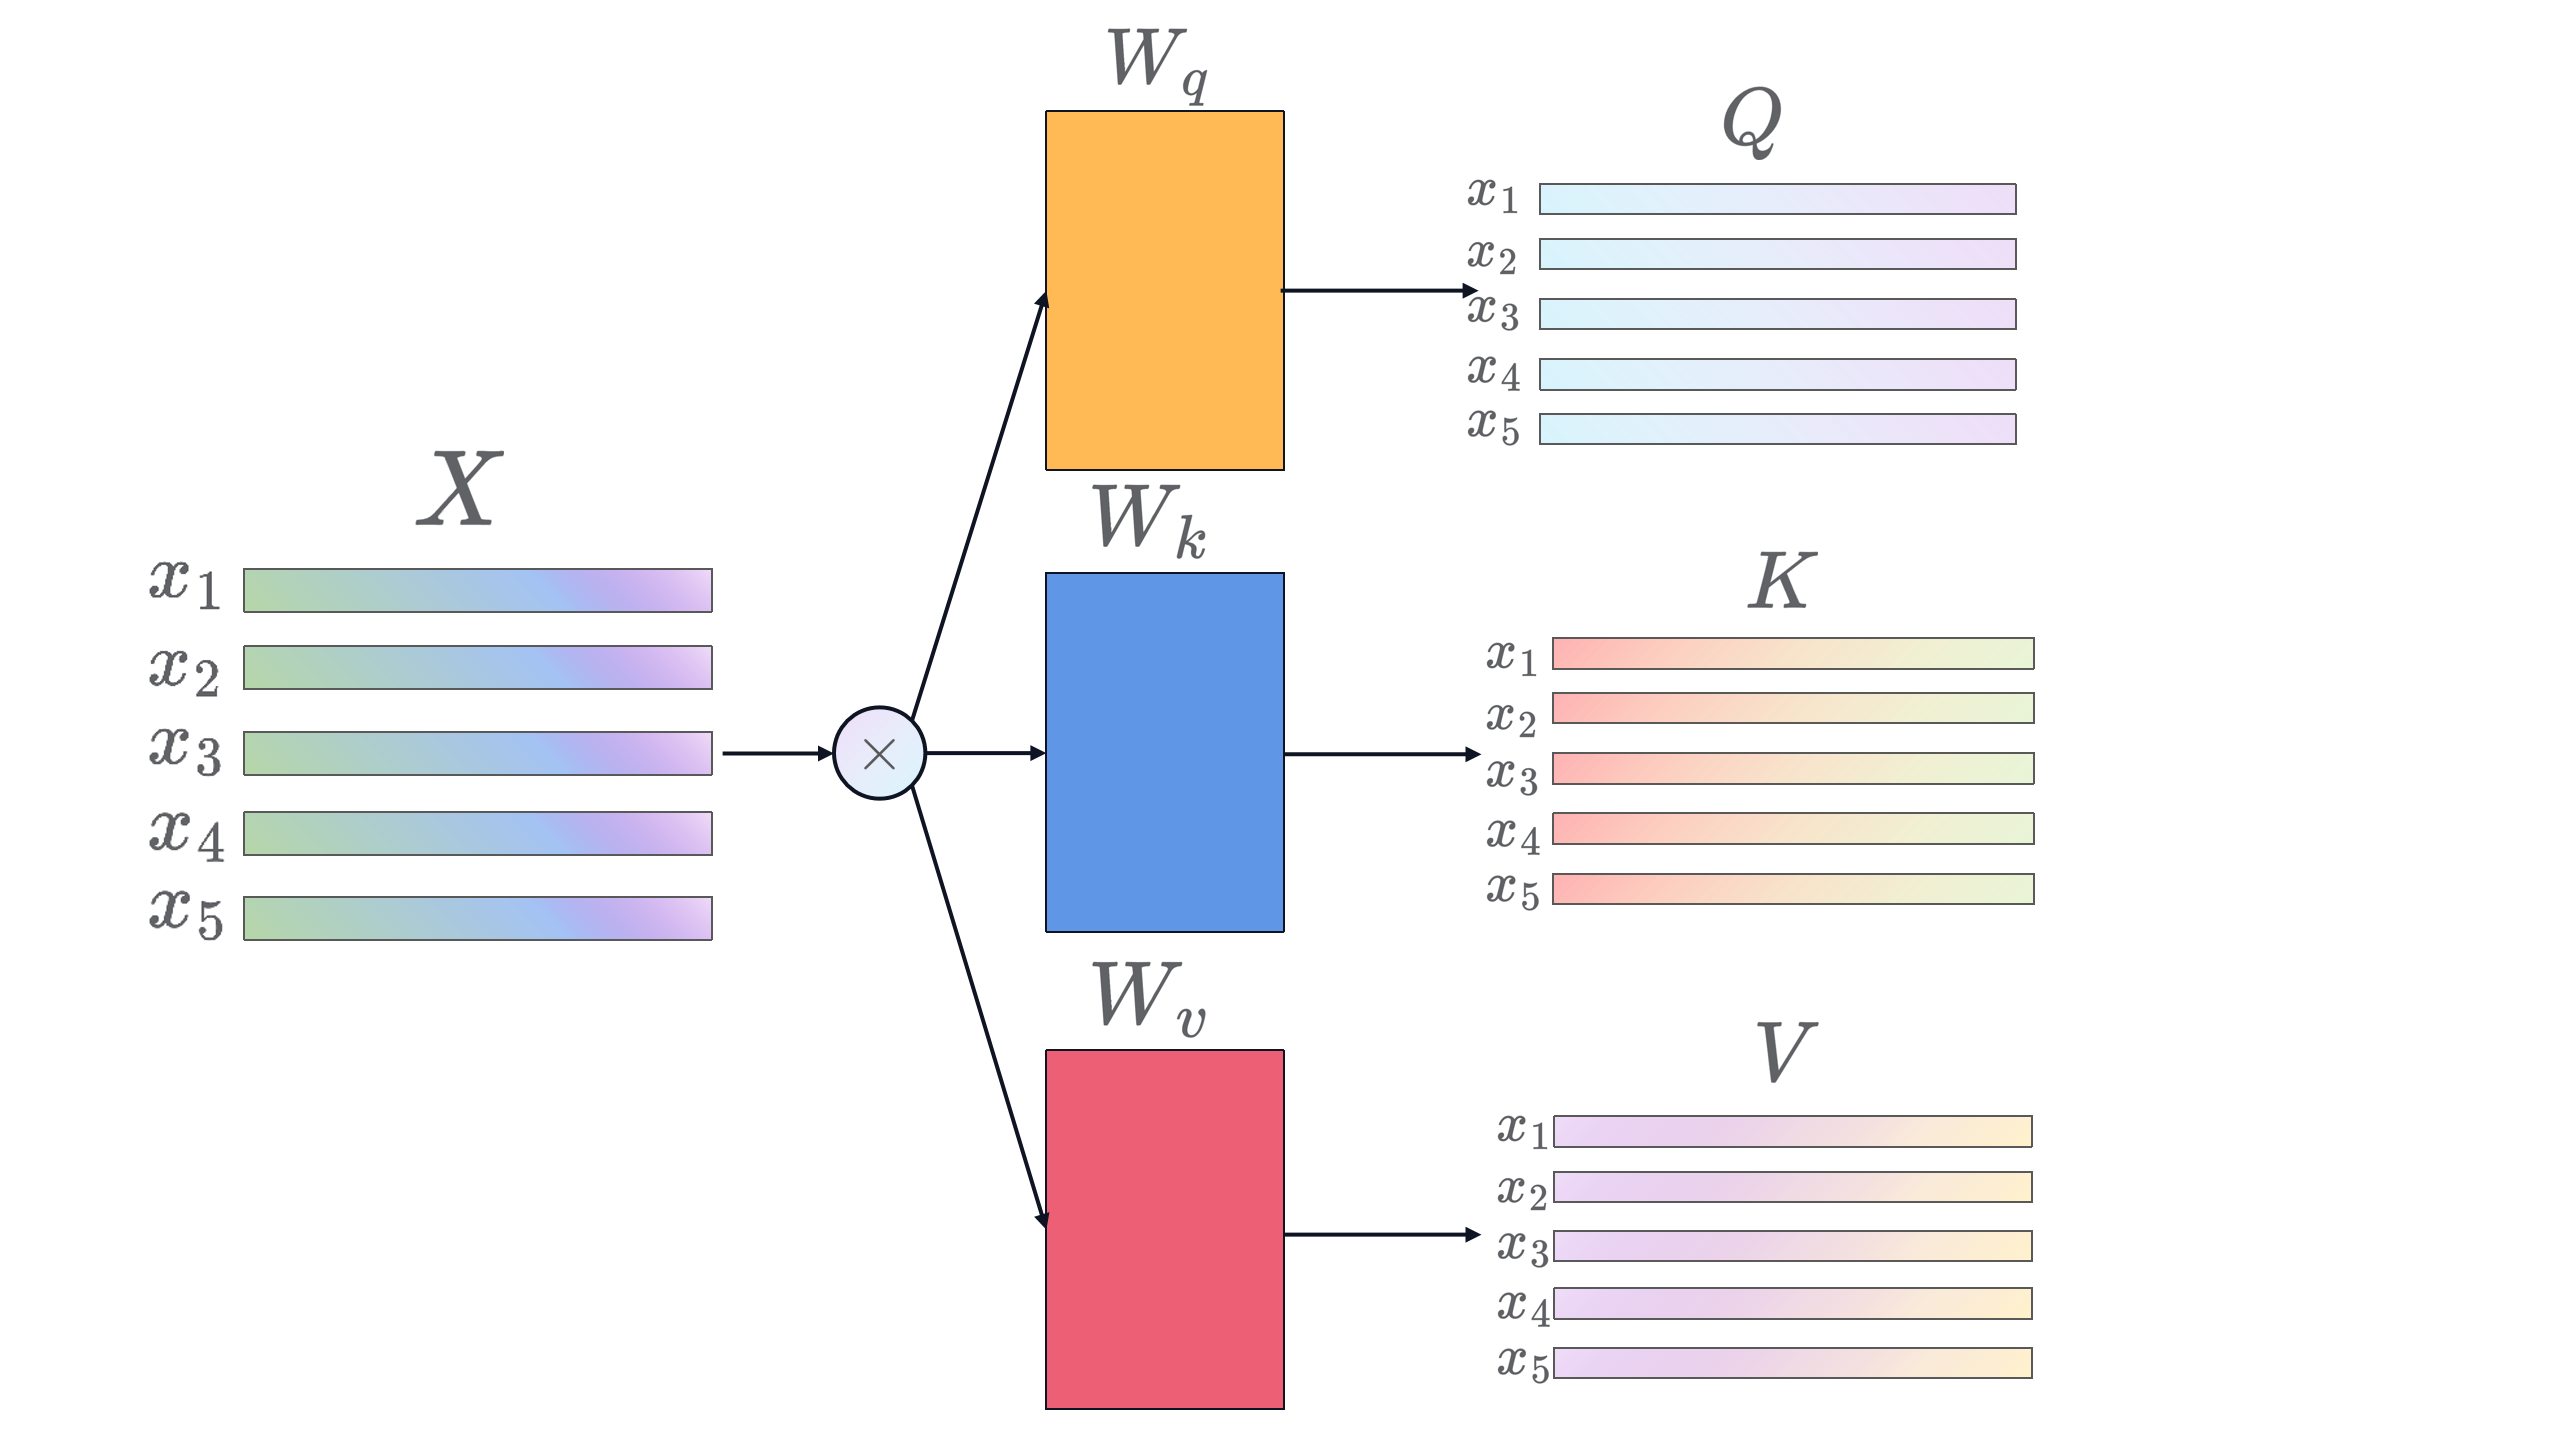
\includegraphics[width=0.75\columnwidth]{image/chap03/img308.png}
	\caption{将X经过三个线性变换后得到Q、K、V}
	\label{img308}
\end{figure}

\begin{figure}[h]
	\begin{minipage}[t]{0.5\linewidth}
		\centering
		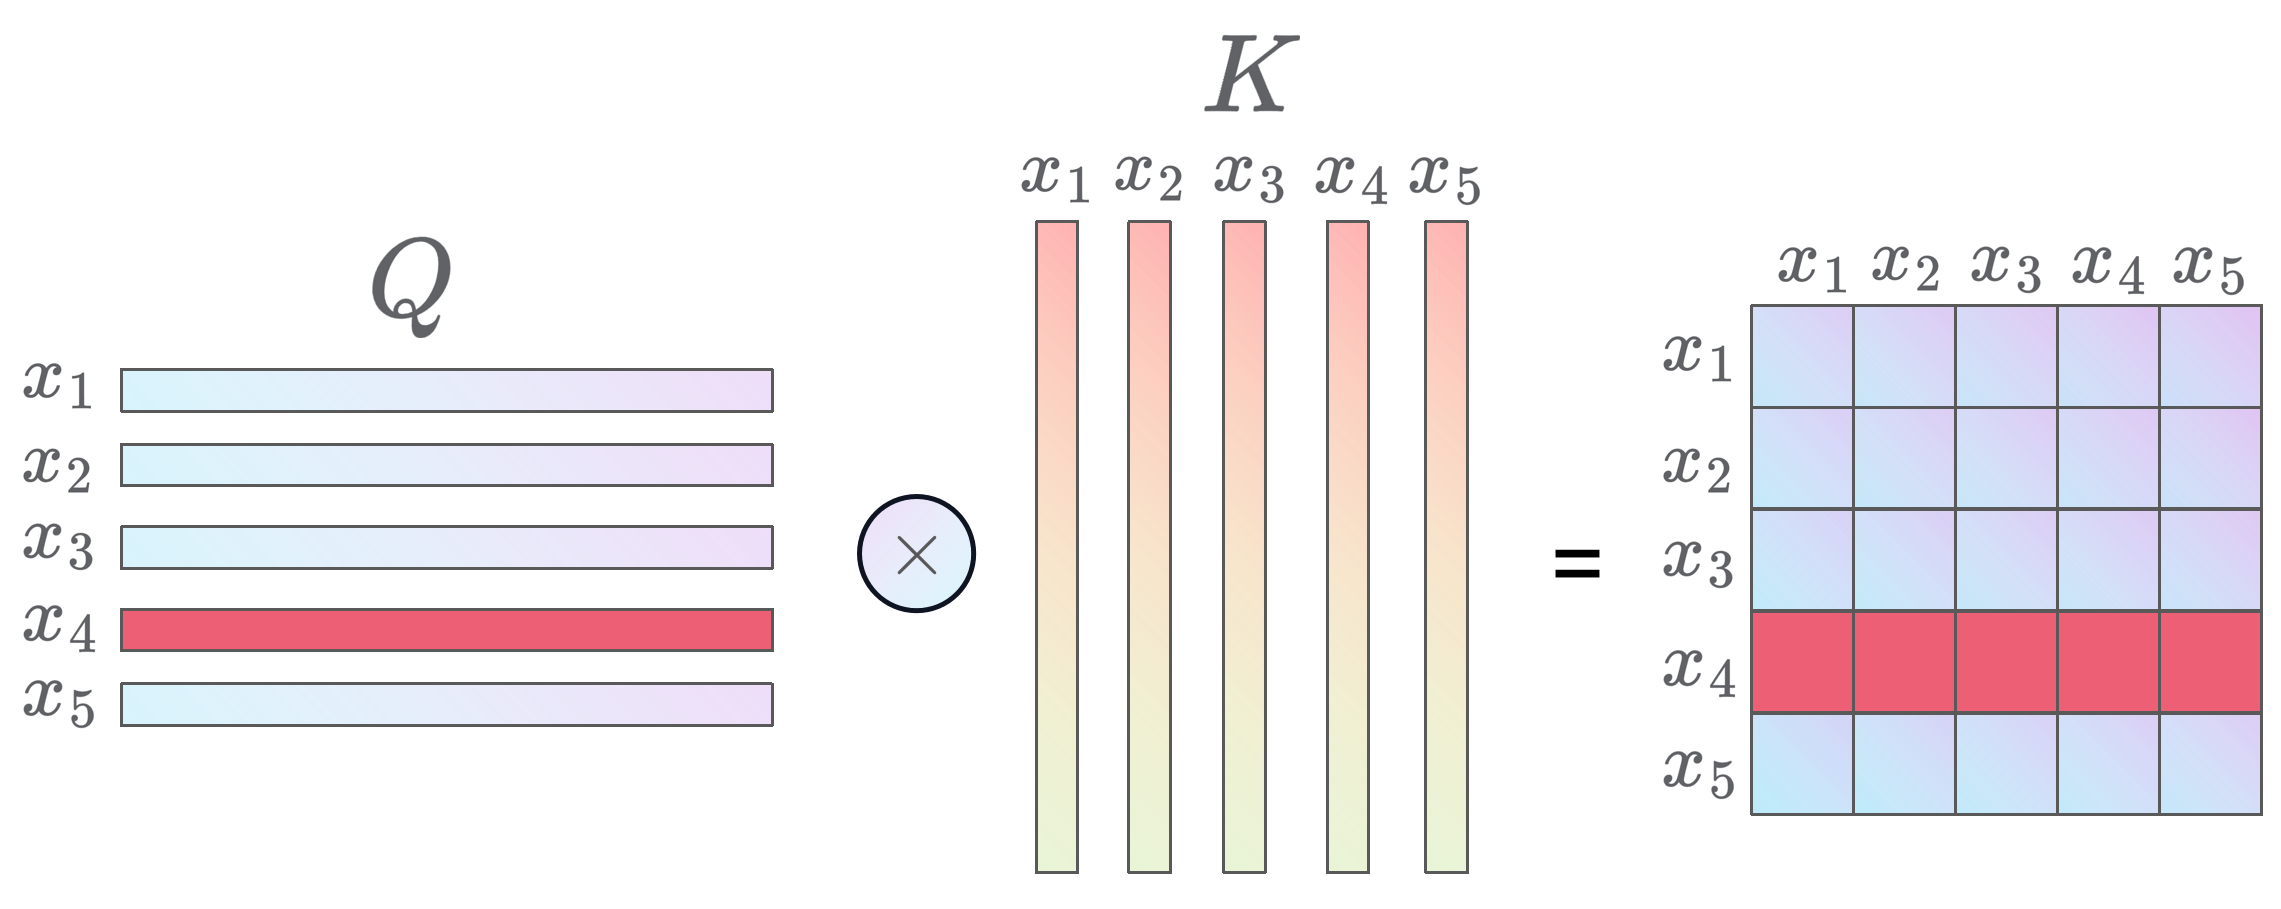
\includegraphics[scale=0.25]{image/chap03/img309.png}
		\caption{Q与K的转置相乘}
		\label{img309}
	\end{minipage}%
	\begin{minipage}[t]{0.5\linewidth}
		\centering
		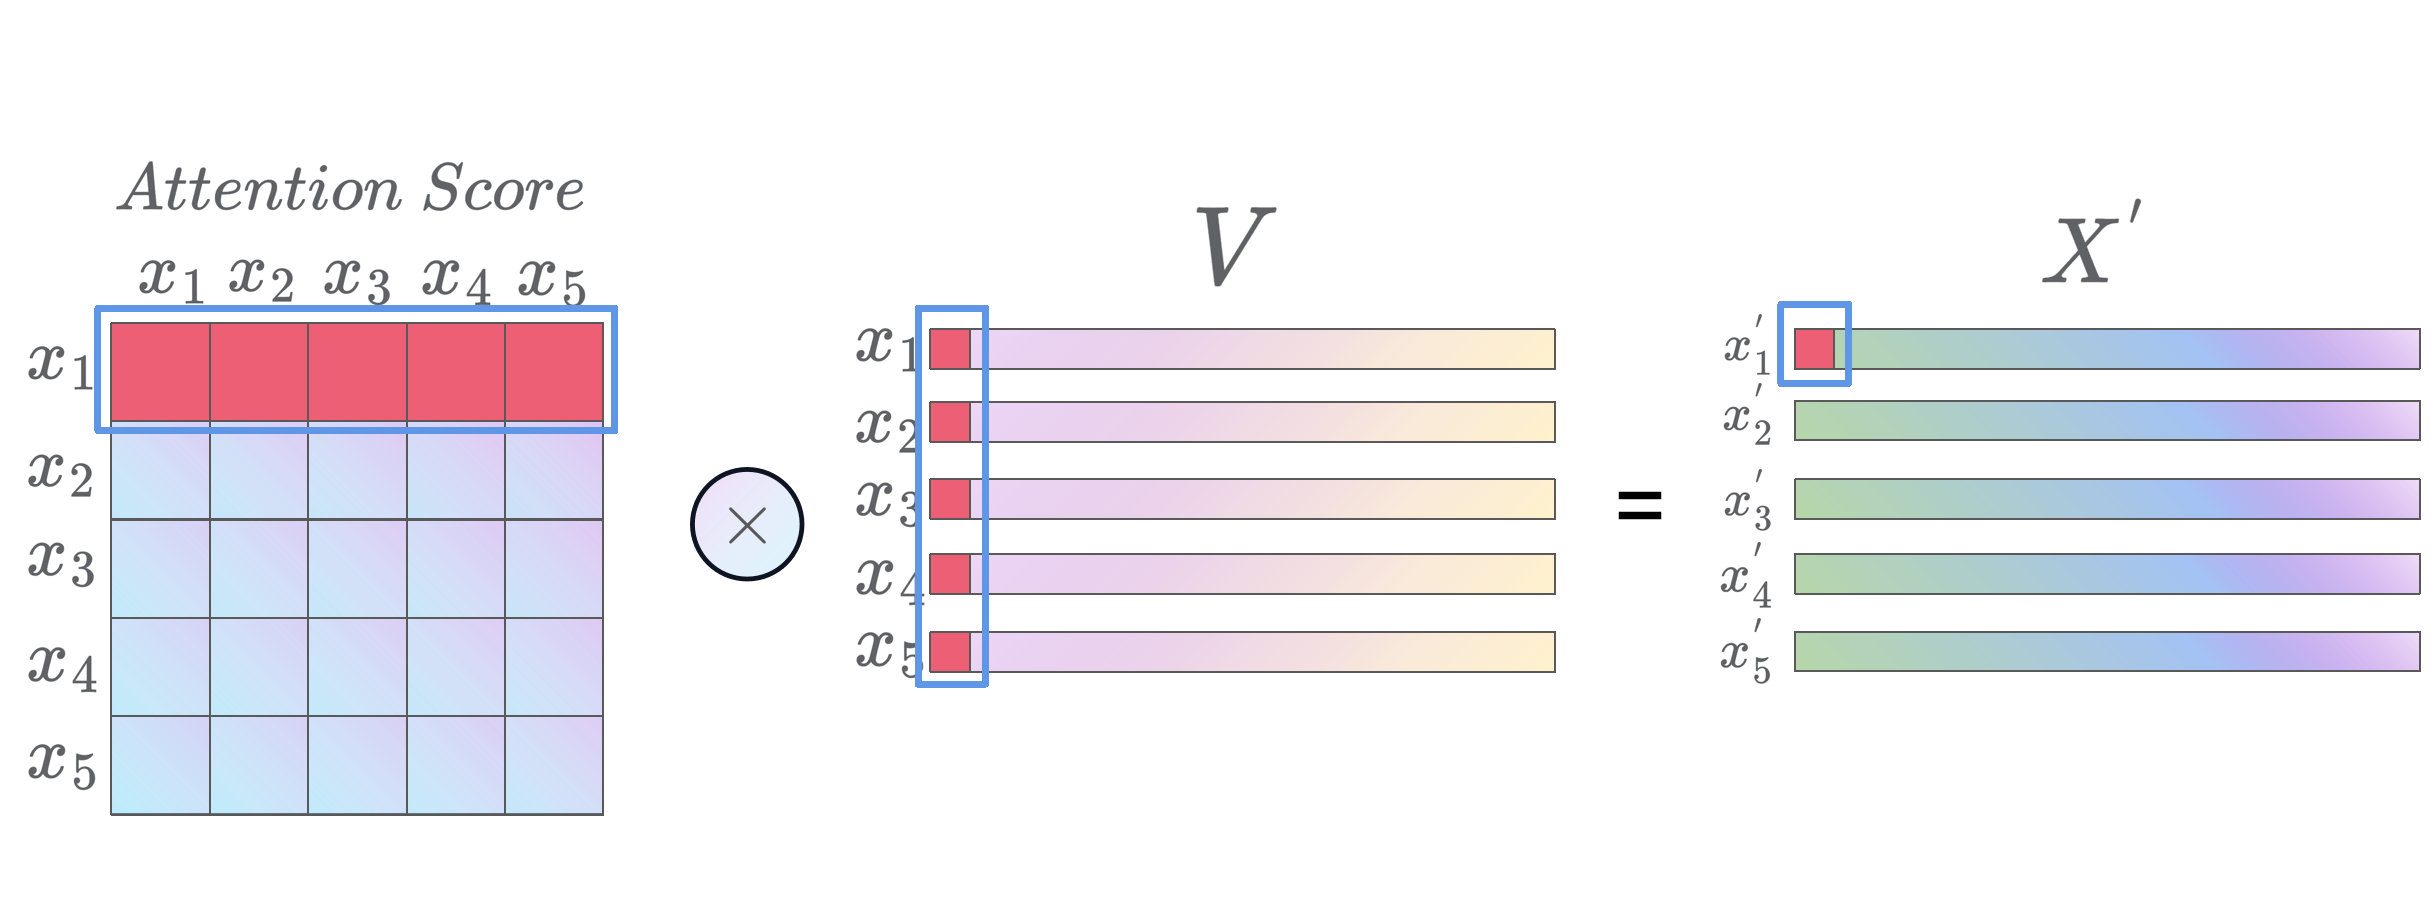
\includegraphics[scale=0.25]{image/chap03/img310.png}
		\caption{将得到的注意力权重矩阵与V相乘}
		\label{img310}
	\end{minipage}
\end{figure}

\subsubsection{将$Q$与$K$输入注意力打分函数得到注意力权重}
其中注意力打分函数的实现如下:

\begin{equation} \label{302}
	\begin{aligned}
		F(X)=softmax(\cfrac{QK^T}{\sqrt{D_k}})
	\end{aligned}
\end{equation}

注意力打分函数的运算由两部分组成:

\begin{itemize}
	\item [1)]
	第一部分是将$Q$与$K$的转置相乘,得到一个矩阵。该矩阵的第i行j列的元素为$x_i$与$x_j$的转置相乘得到的,代表“将$x_i$和$x_j$代入到注意力打分函数”这一操作。如图\ref{img309}所示,右边矩阵红色方块所在行为$Q$中代表$x_4$的行与$K$转置中代表$x_1,x_2,\cdots ,x_5$所在列相乘得到的。
	\item [2)]
	第二部分将所得矩阵各元素进行标准化,而后再进行一次softmax运算。这一步的作用是确保注意力打分函数得到的矩阵各元素都为位于[0,1]之间的权重。运算后得到的矩阵即为注意力权重(Attention Score)矩阵。
\end{itemize}

在图\ref{img303}的机器翻译任务中,第4行1列元素的值代表在翻译“深度”字时,“我”字所提供的信息权重。

\subsubsection{将得到的注意力权重矩阵与$V$相乘}
如图\ref{img310}所示,注意力权重矩阵第一行与$V$相乘得到的$X^{'}$中的第一行元素$x_1^{'}$,可以看作利用所给权重结合$x_1,\cdots ,x_5$信息后的$x_1$。因此最终运算得到的矩阵即代表按照所给权重结合全局信息后的元素$x_1^{'}, \cdots ,x_5^{'}$按行排列而成的矩阵$X^{'}$。

\subsubsection{最终对$X^{'}$再做一次线性变换使之恢复为原来的矩阵形状后输出}
这里所乘的线性变换矩阵$W_0$也为可学习的参数。

综上所述,总体的过程如图\ref{img311}所示。

\begin{figure}[h]
	\centering
	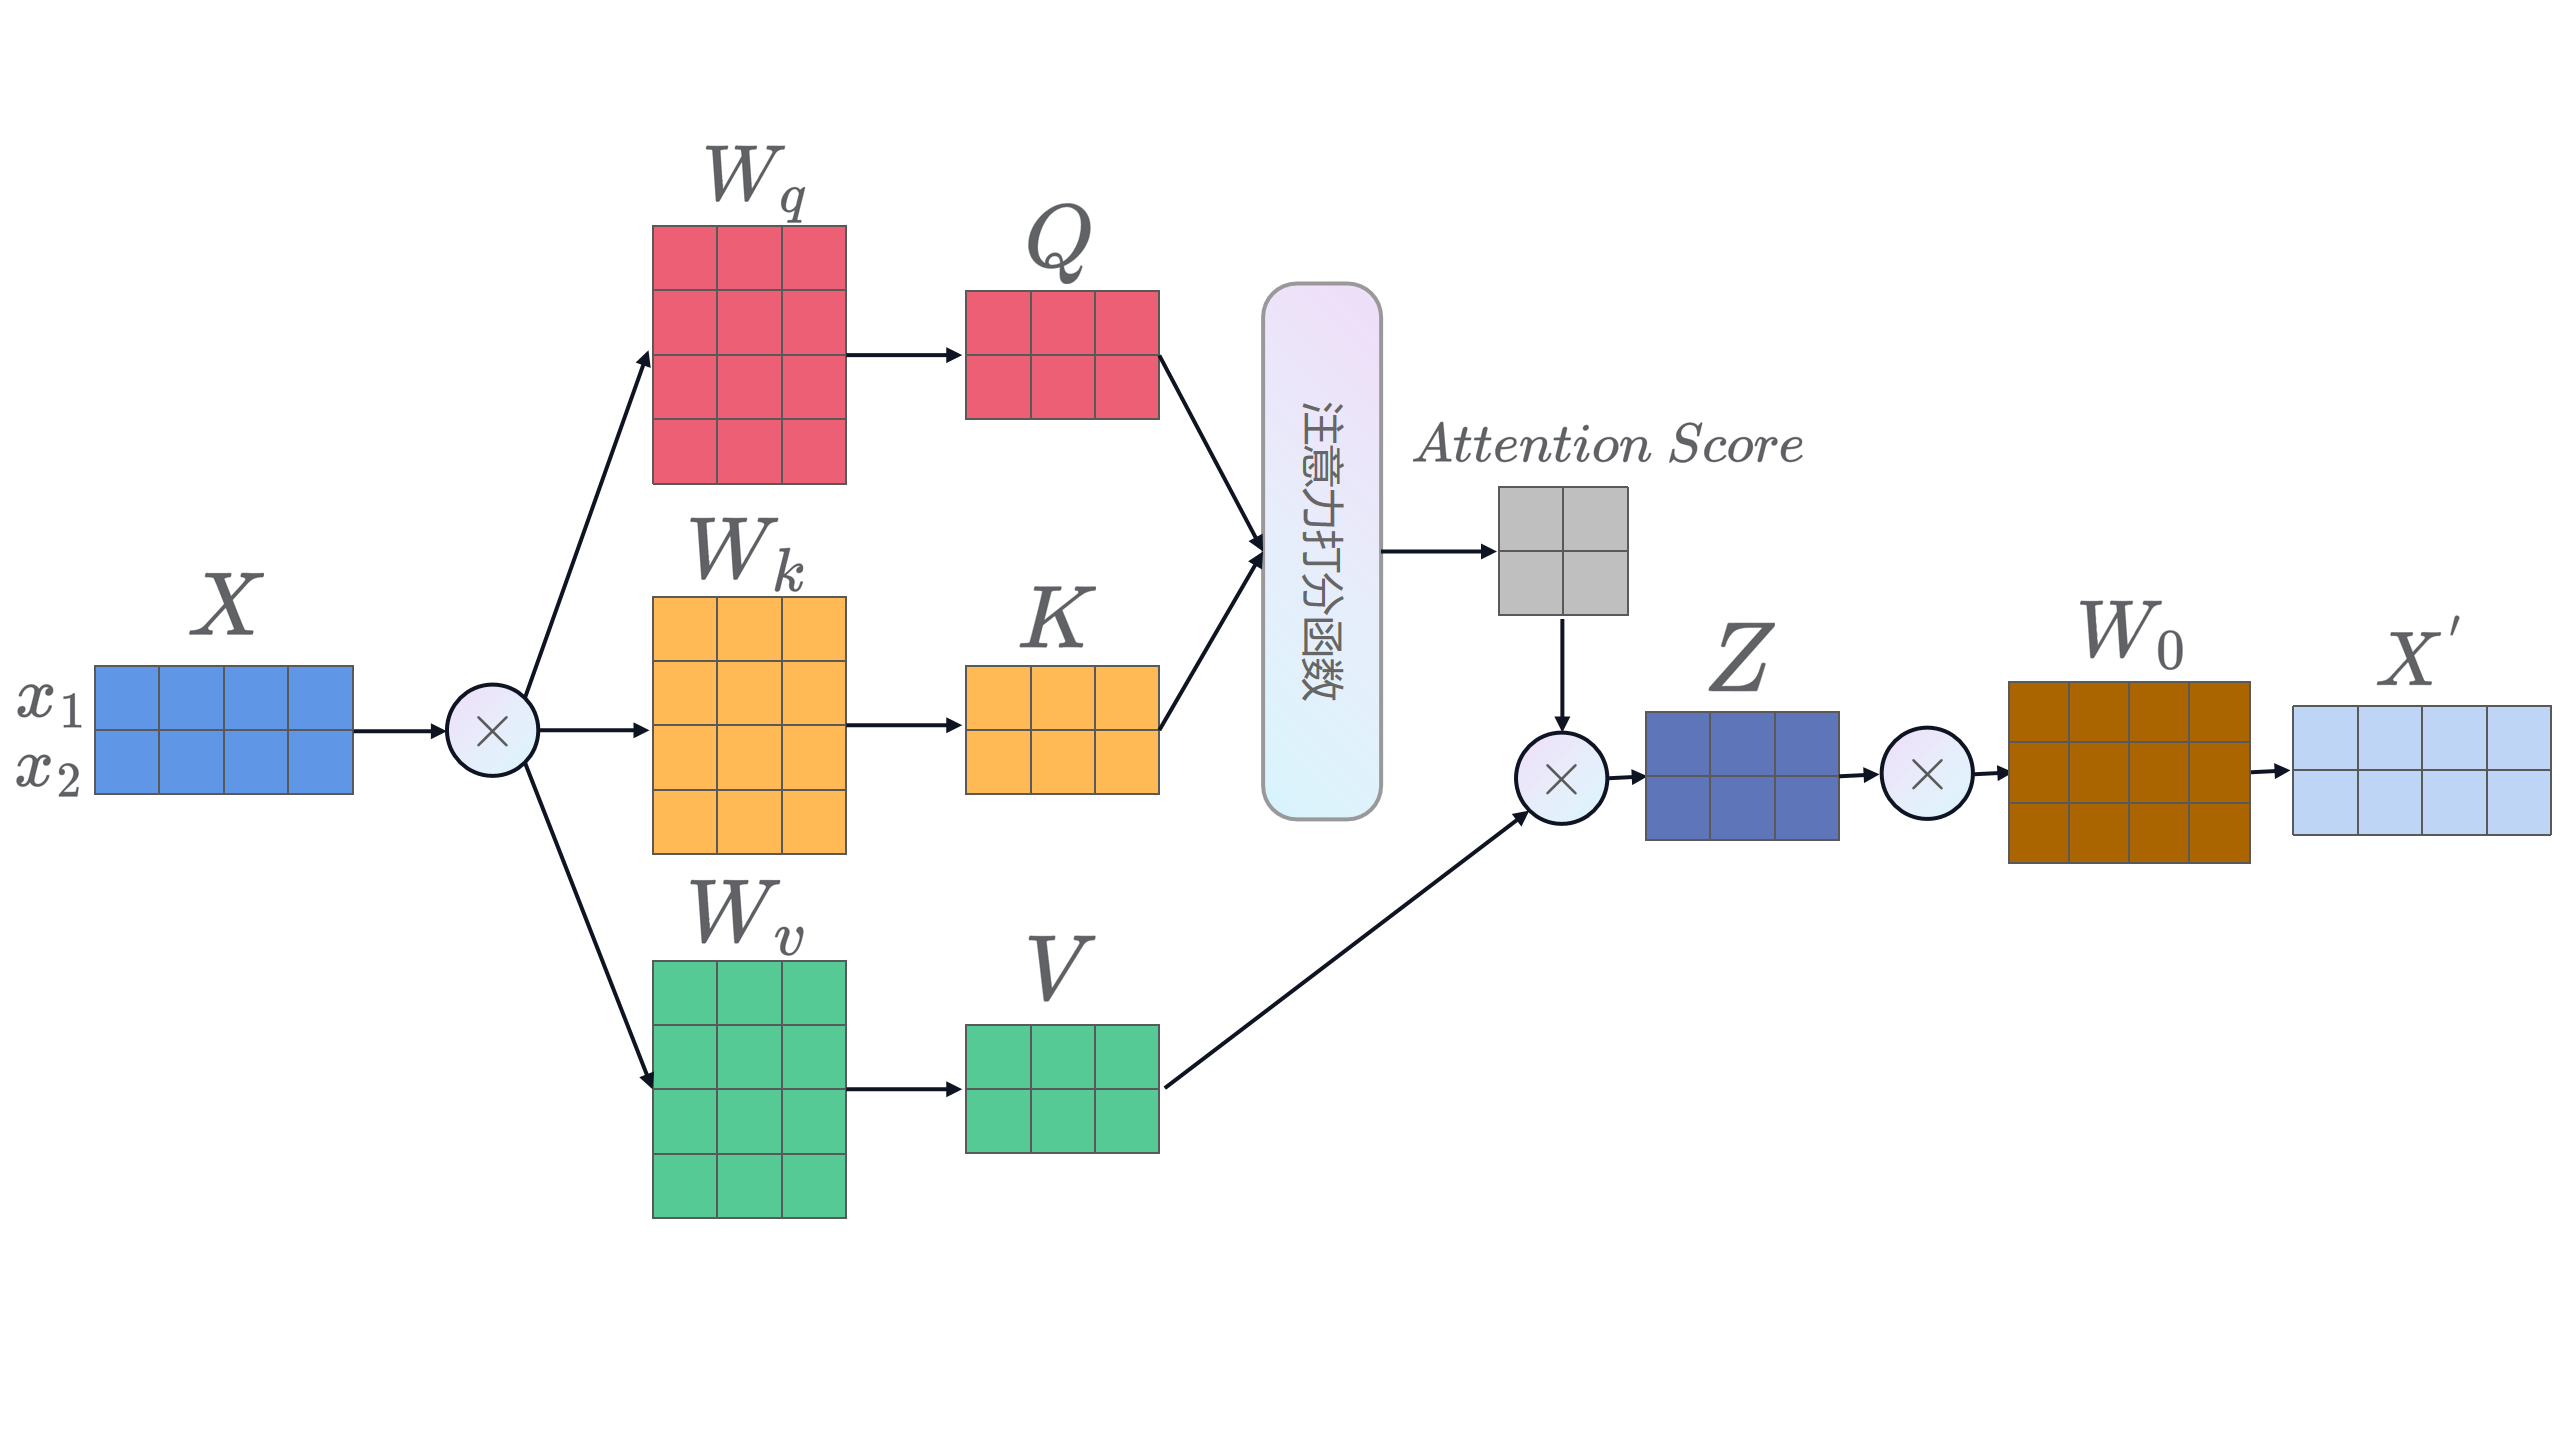
\includegraphics[width=0.75\columnwidth]{image/chap03/img311.png}
	\caption{自注意力机制的实现}
	\label{img311}
\end{figure}

\subsection{多头注意力机制}

\begin{figure}[h]
	\centering
	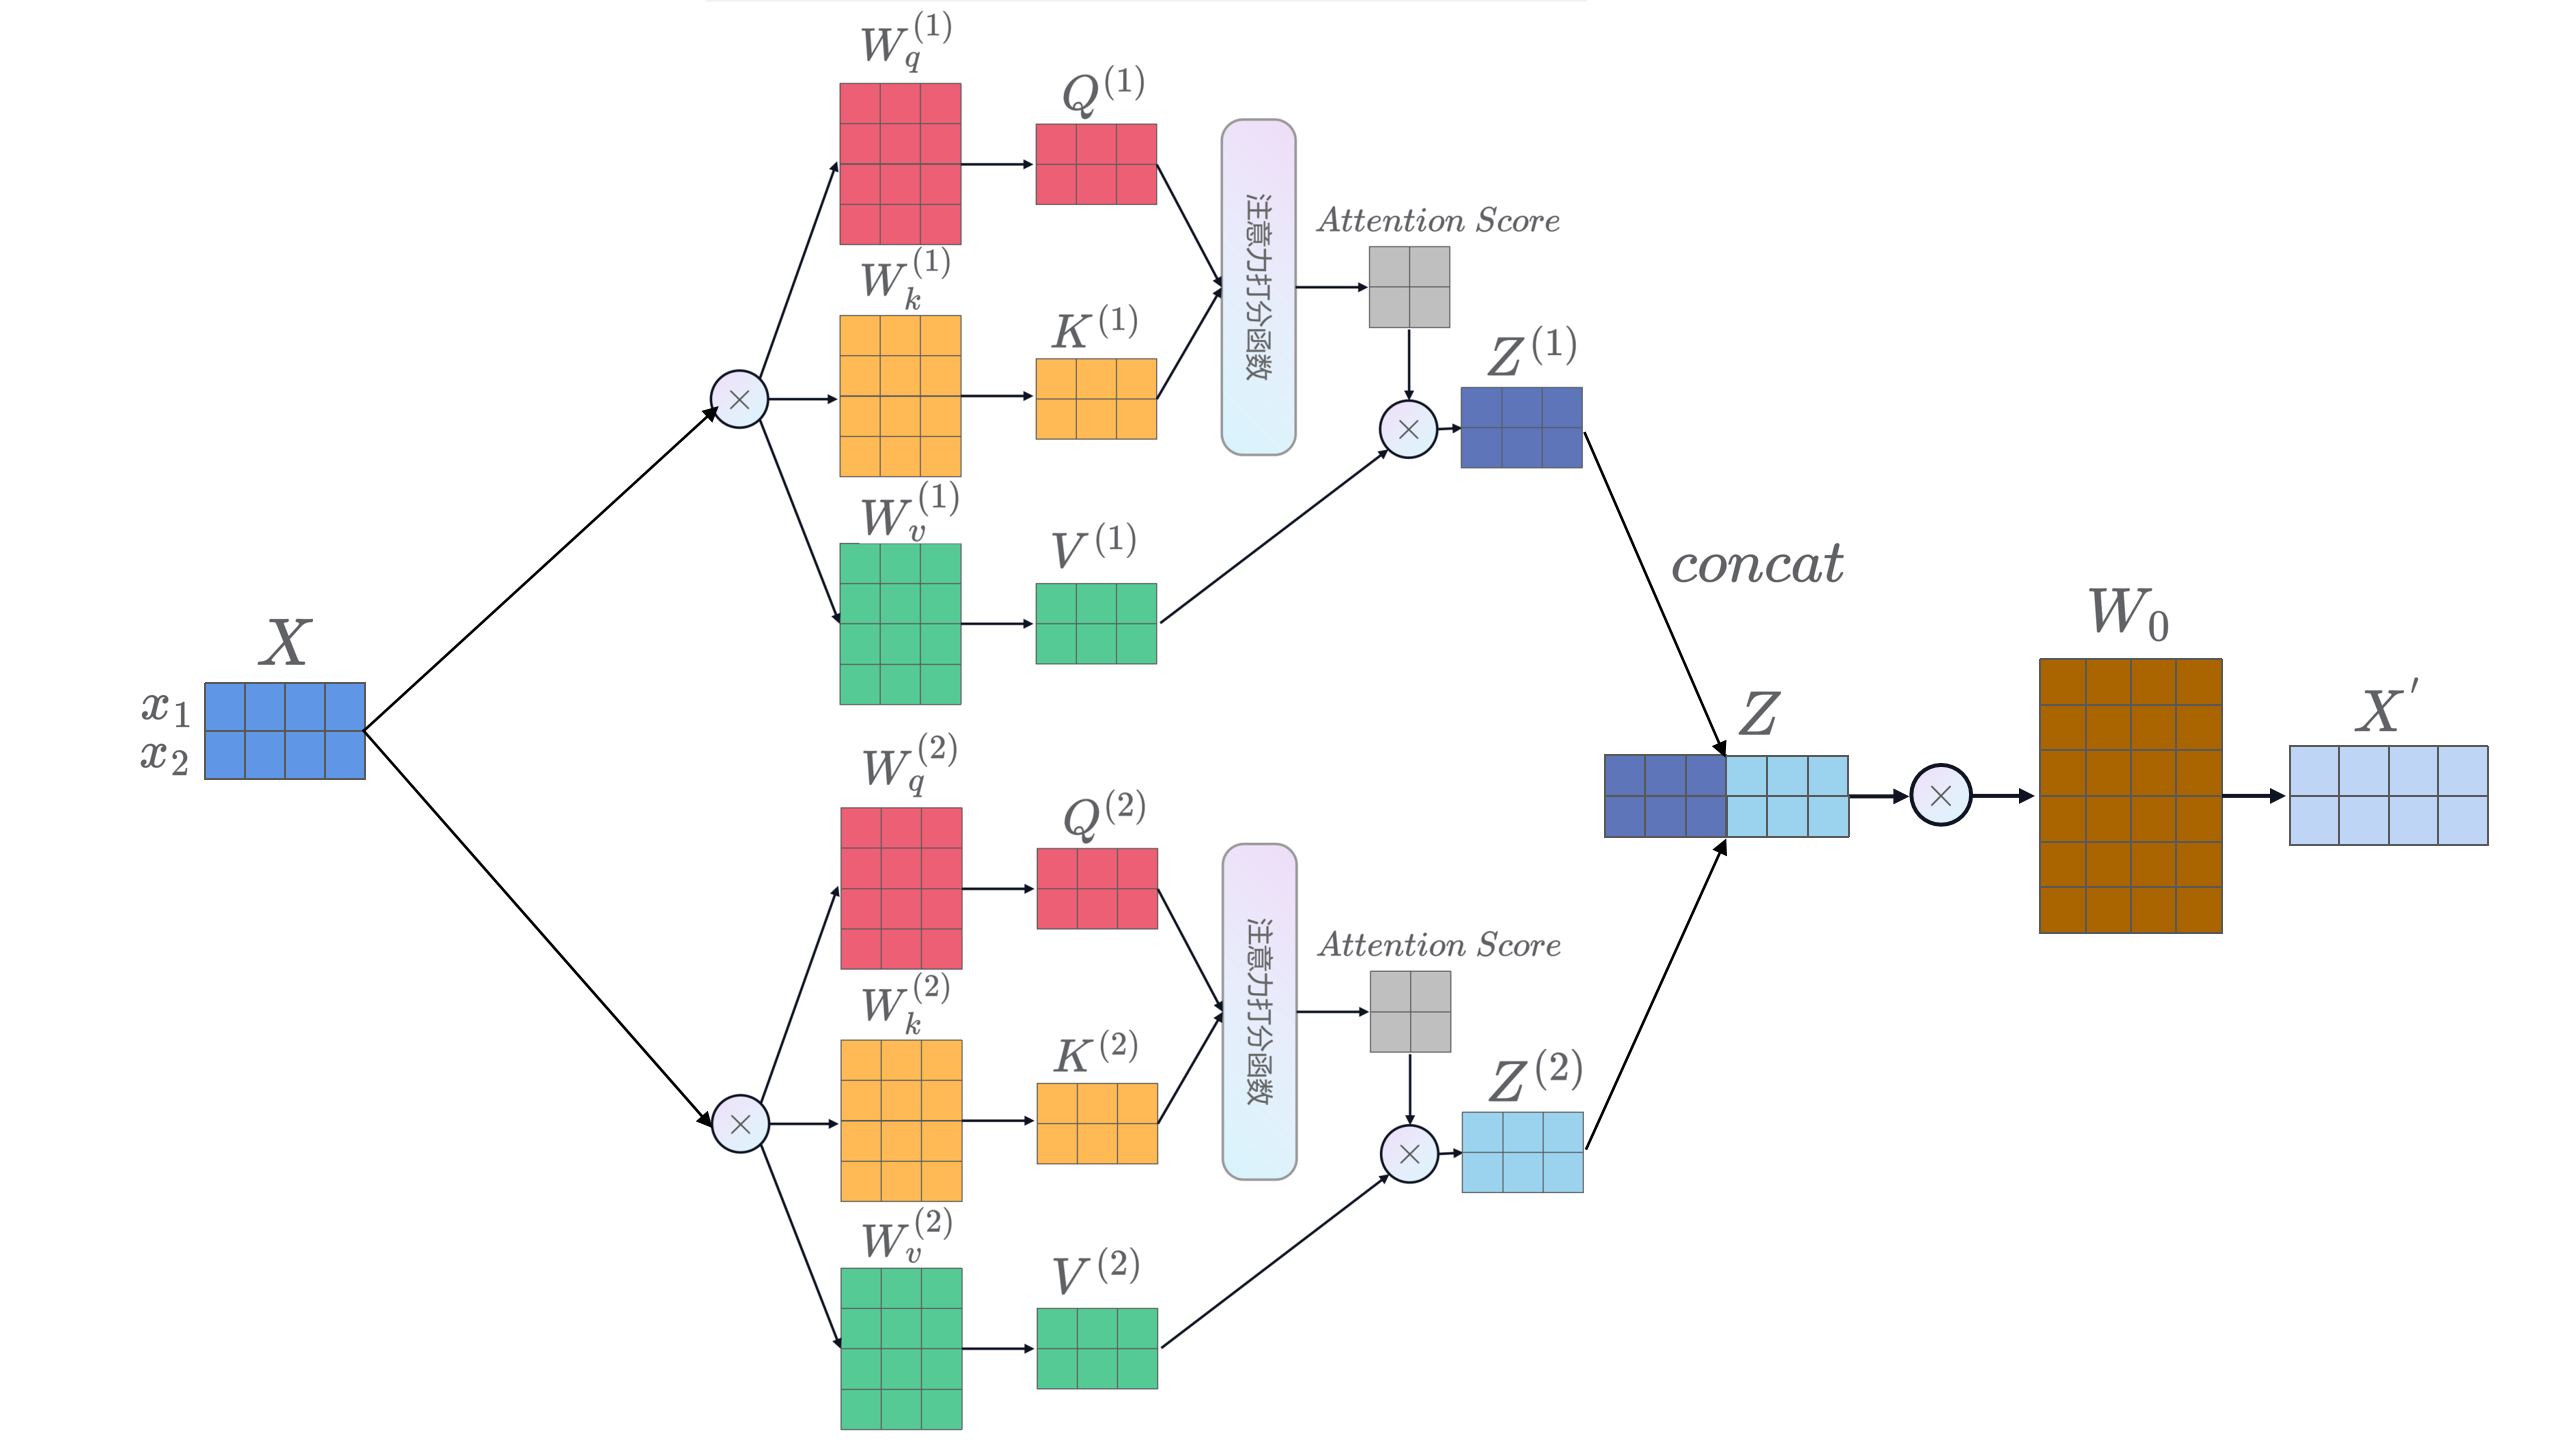
\includegraphics[width=0.9\columnwidth]{image/chap03/img312.png}
	\caption{二头注意力机制的实现}
	\label{img312}
\end{figure}

正如CNN中不同的卷积核能学习到不同的特征,研究人员相信通过增加注意力机制中的注意力打分函数个数,可以让模型学习到不同的信息权重特征,进而优化模型表现。

比如图\ref{img312}所示的二头注意力机制,通过两组线性变化$(W_q^{(1)},W_k^{(1)},W_v^{(1)})$和$(W_q^{(2)},W_k^{(2)},W_v^{(2)})$将$X$映射成两组$Q,K,V$后,通过自注意力机制得到$z^{(1)},z^{(2)}$;将得到的$z^{(1)},z^{(2)}$经过concat连接后,再对其进行一次线性变换,恢复原形状后输出。

其余多头注意力机制的实现与二头注意力机制的实现是相似的,区别仅在于n头注意力机制的注意力打分函数个数为n个。

\section{Transformer在CV领域的应用与改进}
将自注意力机制运用于CV领域是现今Transformer发展的一个重要方向。一张图片由一个个像素点组成,如果直接将Transformer应用在图片上就需要每个像素点跟其他所有像素点都算一下权重。那么一张分辨率为$n*m$的图片就要计算$(n*m)*(n*m$)次注意力机制。随着图片像素的增加,运算的复杂度就会呈现平方级增长。

为了应对这个问题,提出了不同的Transformer模型的改进方法。下面介绍几种典型的改进方法:

\subsection{与卷积相结合的CV Transformer}
在这类模型中,先利用卷积层将图像进行降采样后,使其分辨率降低。然后再将其输入到Transformer中。

\subsection{Axial-Attention(轴向注意力)}
 Axial-Attention对一个像素进行自注意力机制的计算时,不是让它与其他所有像素做注意力机制,而是先只与同行像素做注意力机制后,再与同列像素做注意力机制。在这种改进方法下,单个像素的运算量从原来的$o(n*m)$变成了现在的$o(m+n)$,使得计算量大大降低。
 
 由于第一步的轴向注意力操作能使每个像素点就蕴含了整行的信息,而第二步的轴向注意力操作能使得这些已经蕴含了整行信息的像素点之间进行同列信息的相互结合,于是研究人员认为这种串联的处理方法不仅使得单个像素点能结合所在行与列的信息,而且还能让单个像素点结合整个图象的全局信息。
 
 轴向注意力机制的具体操作如图\ref{img313}。
 \begin{figure}[h]
 	\centering
 	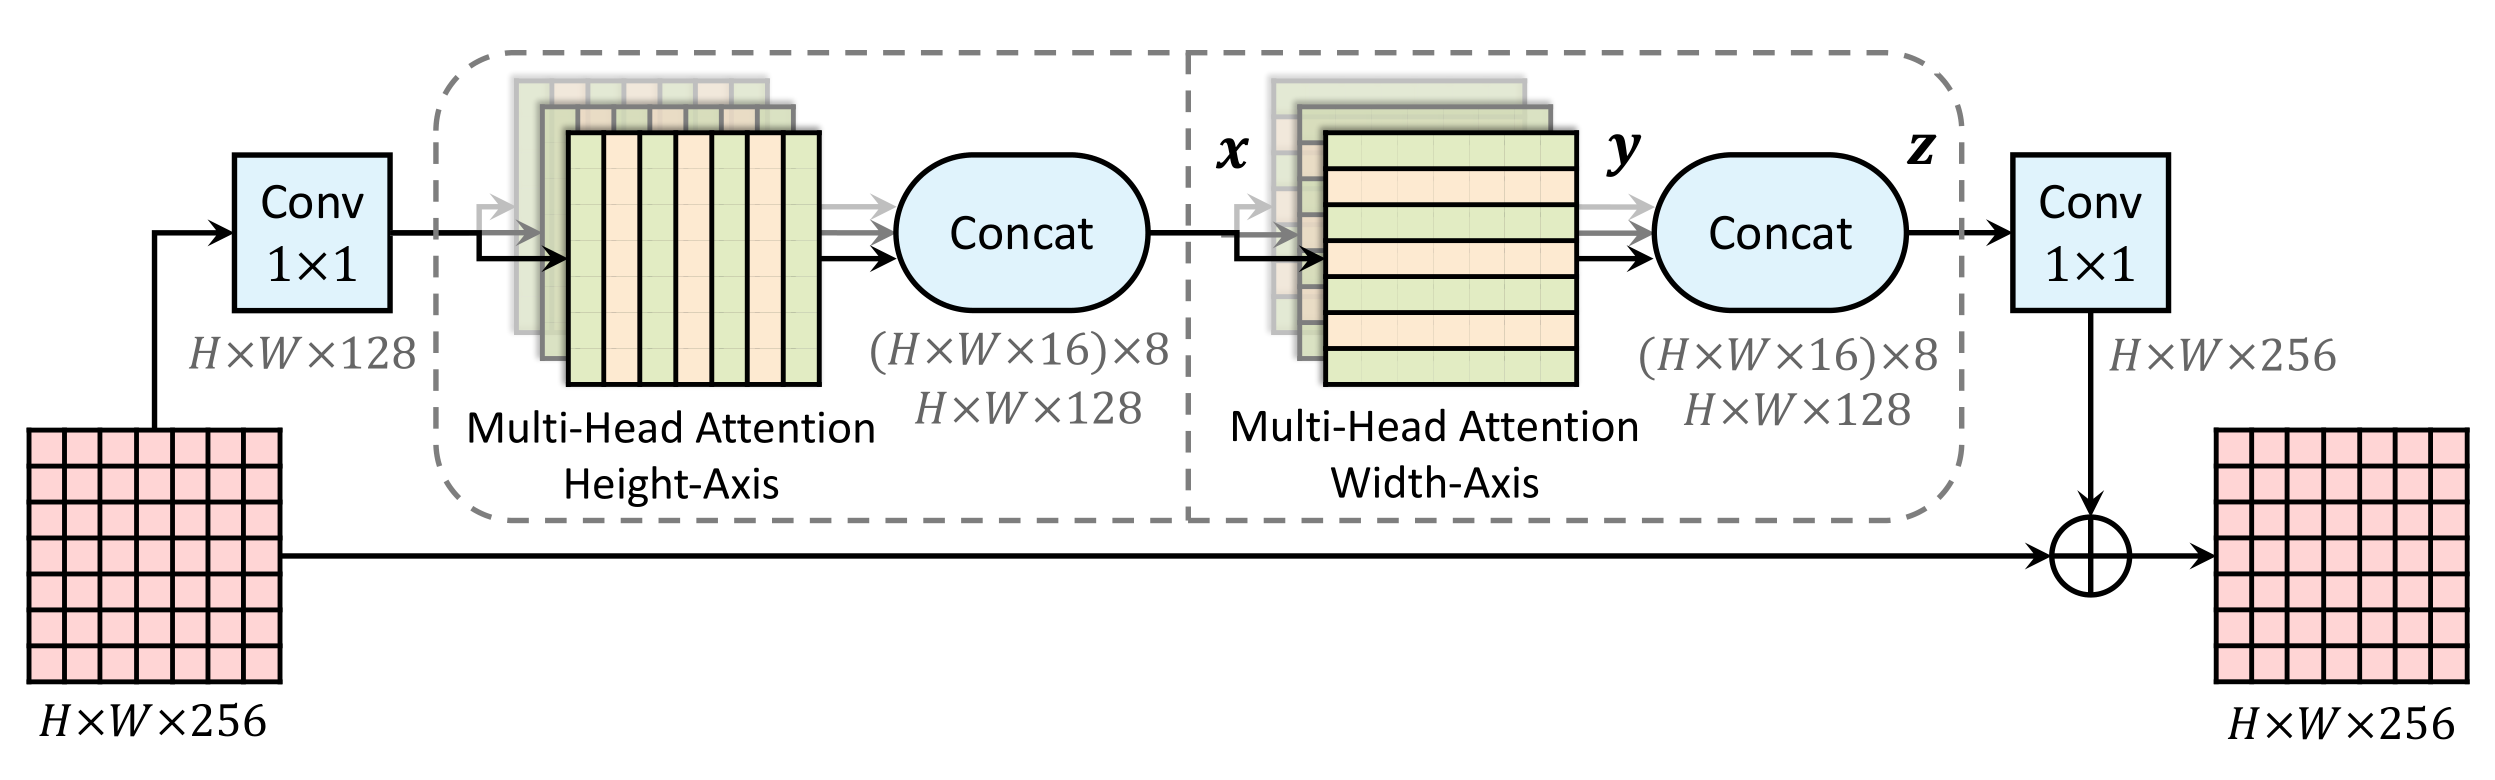
\includegraphics[width=0.75\columnwidth]{image/chap03/img313.png}
 	\caption{Axial-Attention模型的结构\cite{wang2020axial}}
 	\label{img313}
 \end{figure}

\subsection{ViT神经网络对注意力机制的实现}
 ViT神经网络对传统注意力机制的改进方法是把先将图像进行分割,分割成一个个固定大小的patch,将这个patch看成一个大像素(每个patch展平当作一个向量),然后在让所有这些“大像素”向量之间做自注意力机制。这时就等价于对一张更低像素图片做注意力机制,达到将计算量变少的目的。具体ViT神经网络的实现如图\ref{img314}所示。
 
 \begin{figure}[h]
 	\centering
 	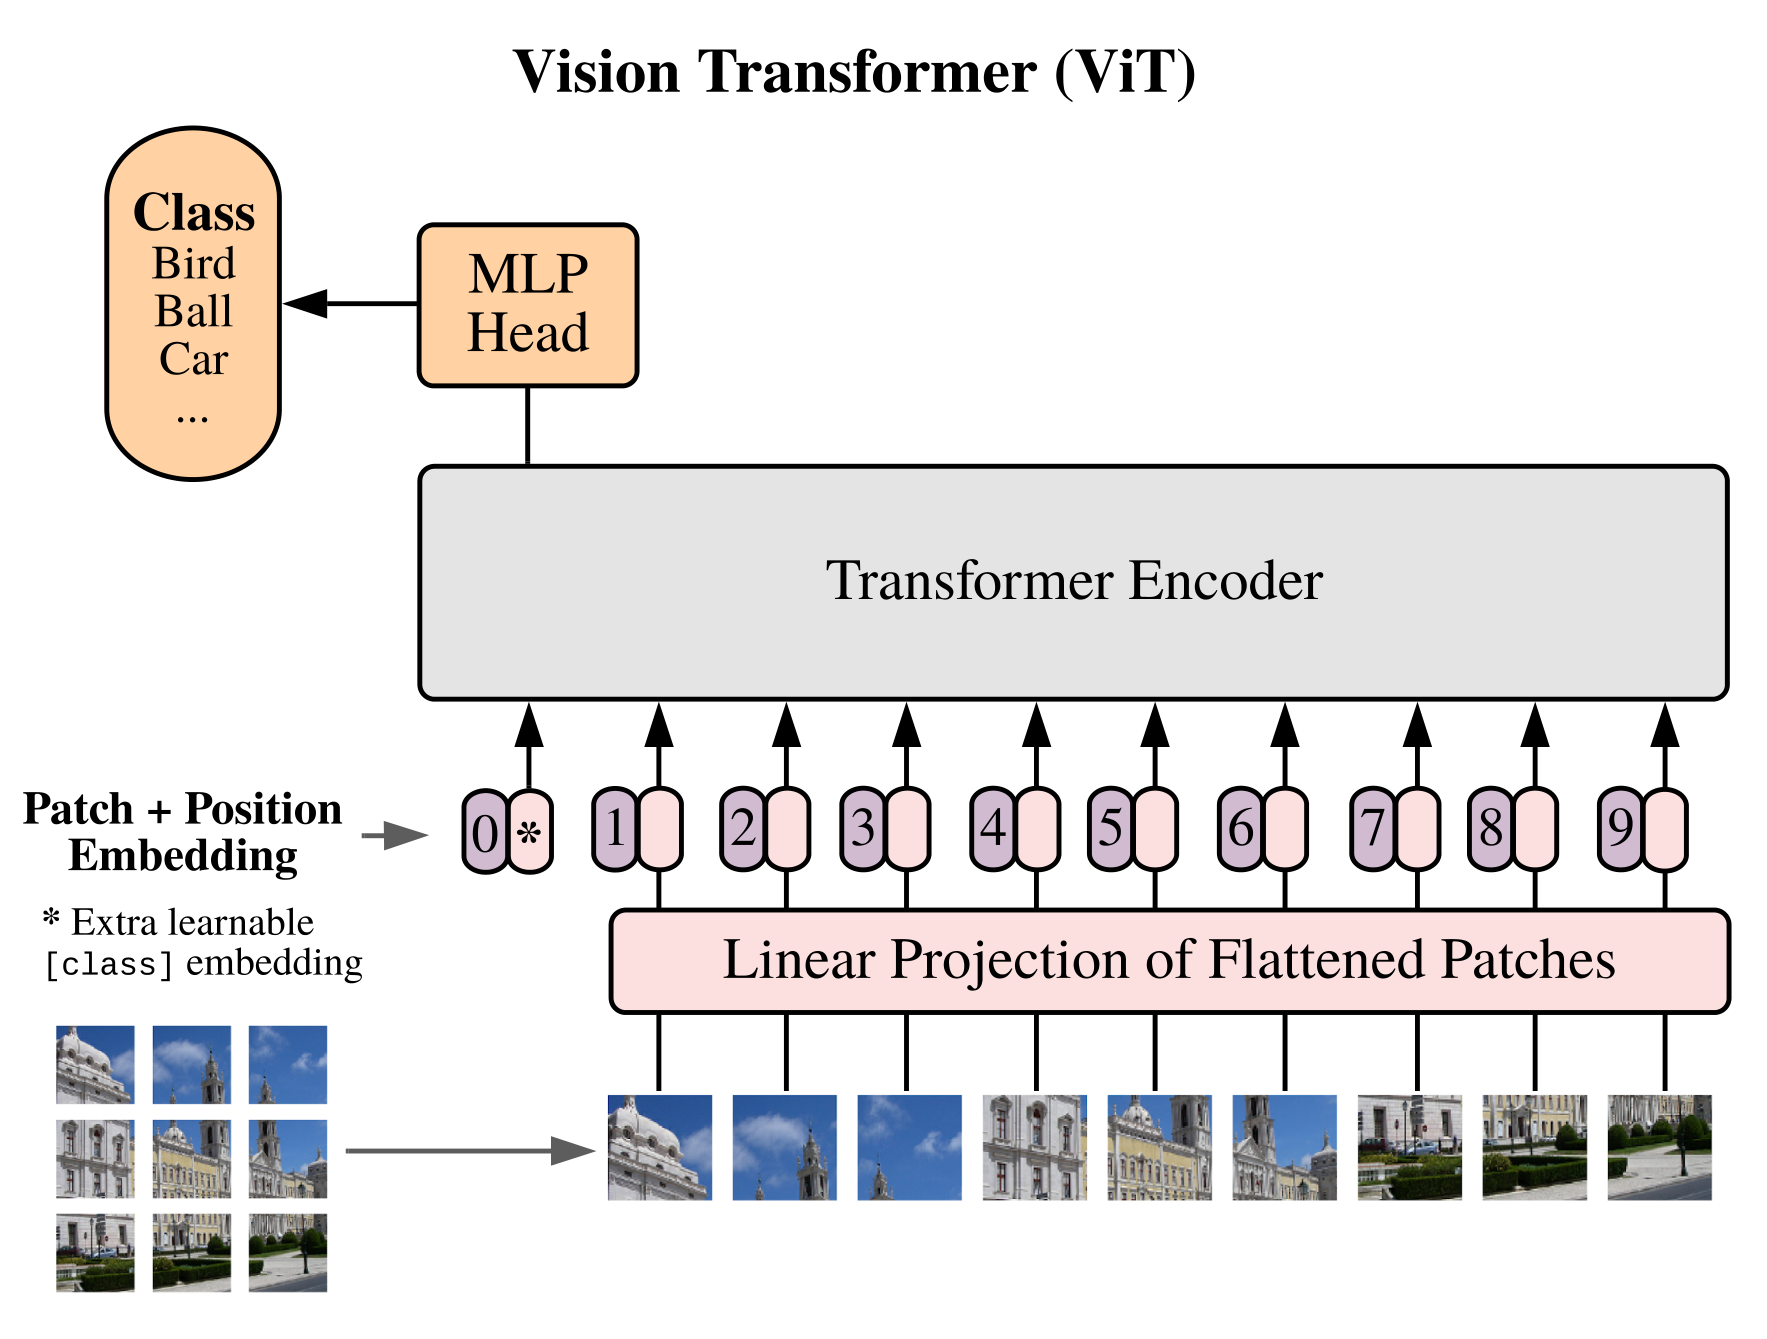
\includegraphics[width=0.5\columnwidth]{image/chap03/img314.png}
 	\caption{ViT模型的结构\cite{dosovitskiy2020image}}
 	\label{img314}
 \end{figure}

\hspace*{\fill} \

\hspace*{\fill} \

\hspace*{\fill} \

\hspace*{\fill} \

\subsection{Swin Transformer}
与ViT的改进不同,Swin Transformer在将图像进行分割成patch后,并不是在这些patch间运算注意力机制,而是对patch内的各像素间做注意力机制。这部分操作是在W-MSA内完成的(即W-MSA(Window Attention):分成一个个patch,然后在patch内部做自注意力机制,做完后再拼接到一起)。虽然这样运算能因像素点减少而使得运算量降低,但由于patch与patch是相互独立,缺乏联系的,而导致单个像素无法很好地融合整个图像的信息。

于是Swin Transformer在W-MSA完成后又引入了SW-MSA操作,即采用滑动窗口后的再分割来规避上述缺陷。具体操作见图\ref{img315}。

 \begin{figure}[h]
	\centering
	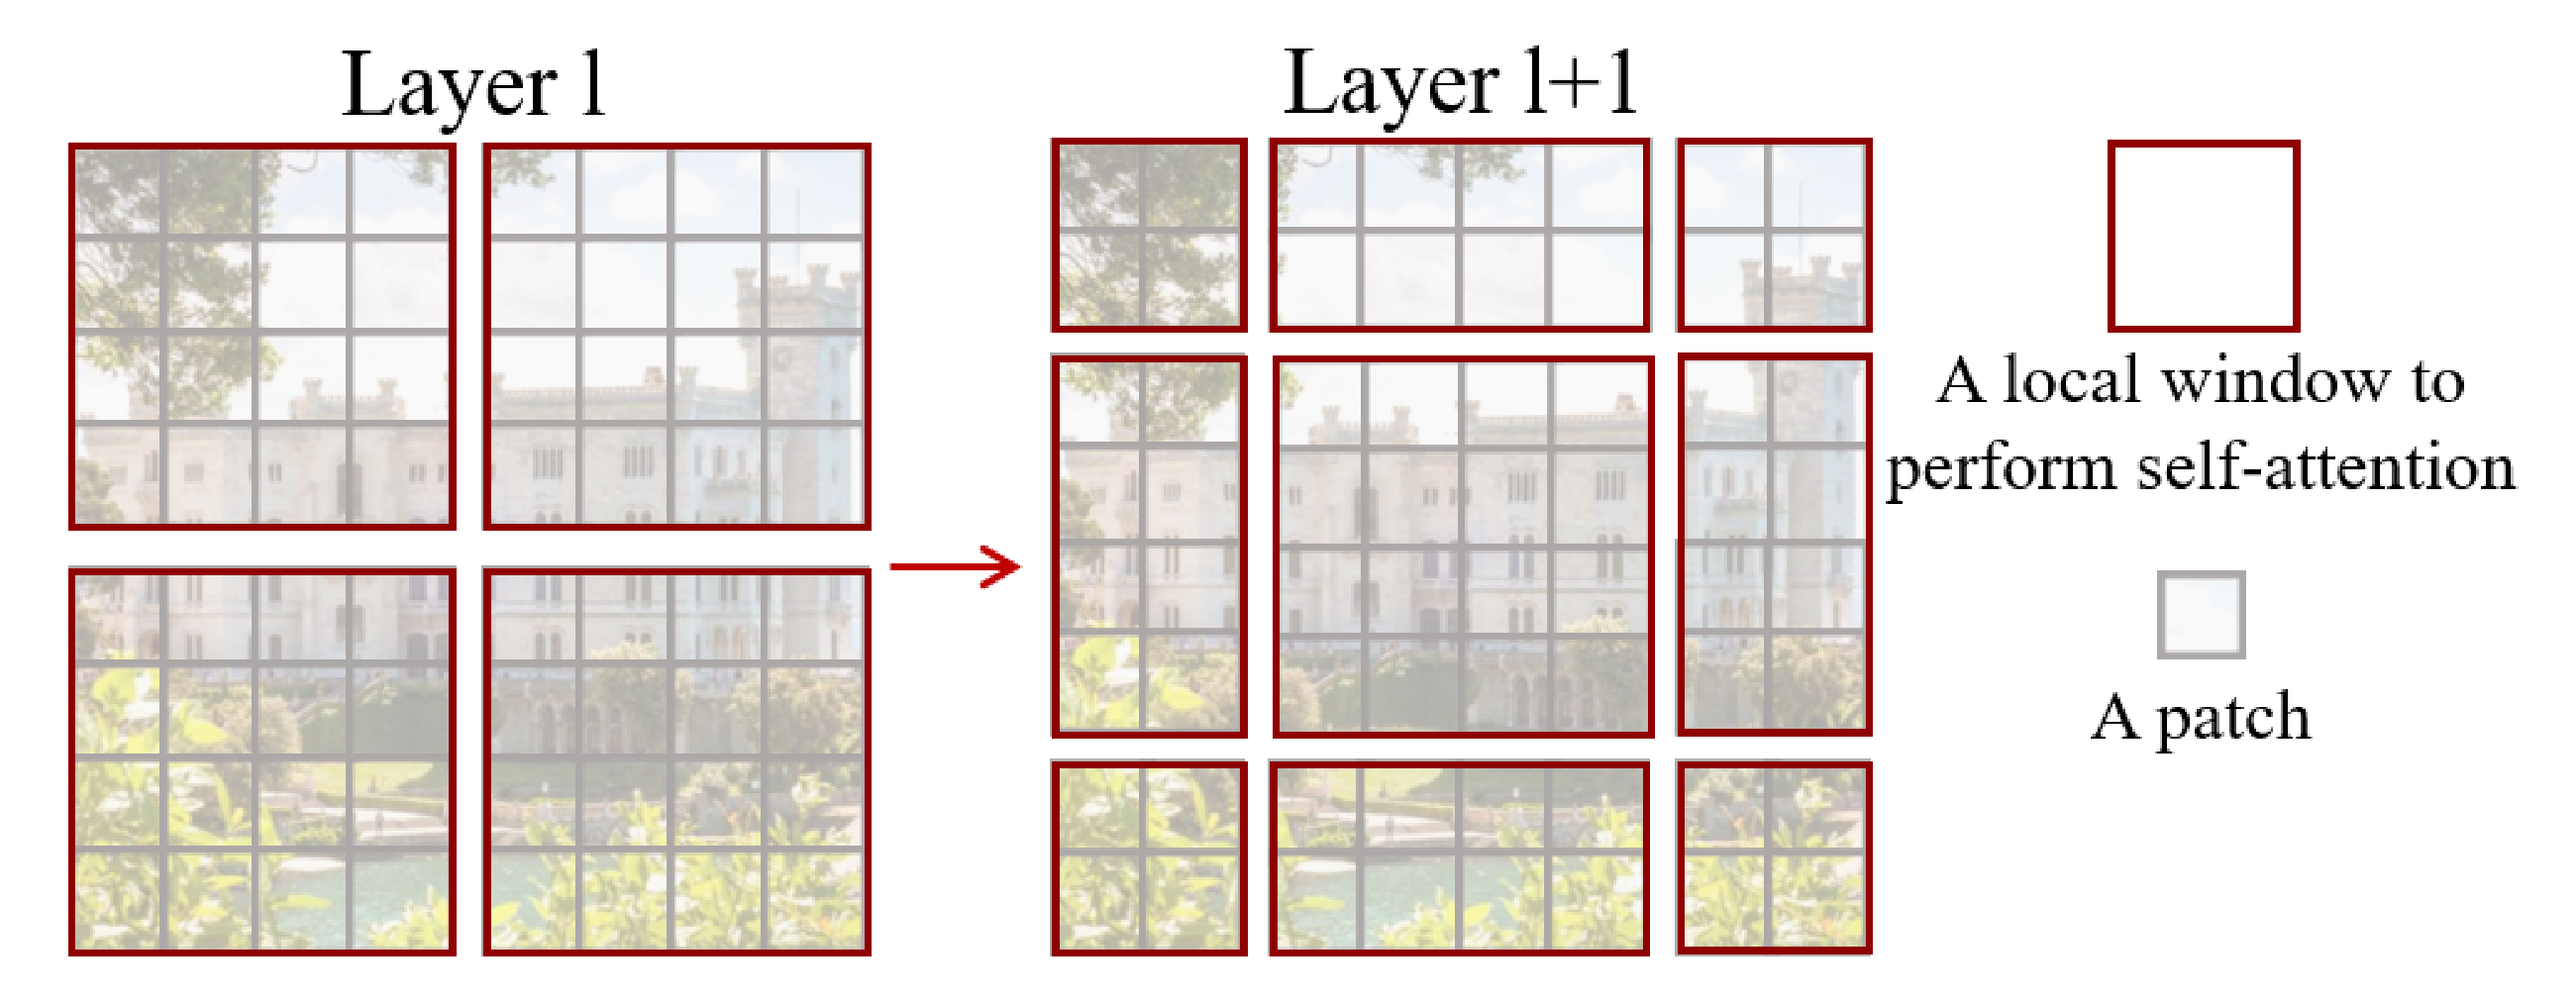
\includegraphics[width=0.75\columnwidth]{image/chap03/img315.png}
	\caption{Swin Transformer中的SW-MSA操作\cite{liu2021swin}}
	\label{img315}
\end{figure}
 
 如图\ref{img315}所示,整个过程是首先由W-MSA做上图左边四个patch的自注意力;然后采用滑动窗口的再分割得到上图右边的9个patch,再在这九个patch内部进行自注意力的运算。此时经过SW-MSA的操作后就使得单个像素能更好的融合整个图像的信息。
 
 \section{SwinTransformer的优势}
 在上述四种改进方法中,Swin Transformer模型在图像分类、目标检测、图像分割等常见的CV领域都有更好的实现效果。经过分析,Swin Transformer模型相较于其他现有模型的优势可能存在如下几点:
 
 \begin{itemize}
 	\item [1)]
 	Swin Transfomer的W-MSA和SW-MSA设计使其计算复杂度为输入图像大小的线性计算复杂度,相较于其他模型显著降低。
 	\item [2)]
 	Swin Transfomer的Patch Merging层设计使得输入图像的分辨率随着层数的加深而不断减小,进而进一步降低整个模型的计算复杂度,使得更深层数神经网路模型的实现成为可能。而深层模型相较于浅层模型往往具有更好的效果。
 	\item [3)]
 	从每个patch的感知范围的角度,Swin Transformer中的层次化构建方式类似于CNN,在逐层缩小图片分辨率的同时,使得每个patch的感知范围扩大。而ViT等改进方法中每个patch的感知范围是固定的。
 \end{itemize}

由于Swin Transformer模型在CV领域具有良好的表现,本项目采用Swin Transformer模型的改进思路来实现将低精度光声重建图像优化为高精度光声重建图像的模型。